\documentclass[12pt]{book}
\usepackage[T1]{fontenc}
\usepackage[utf8]{inputenc}
\usepackage[a4paper, left=2.8cm, right=2.0cm, top=3.0cm, bottom=3.0cm]{geometry}
\usepackage{amsmath, amssymb, amsfonts, amsthm}
\usepackage{ dsfont }
\usepackage{float}
\usepackage{color}
\usepackage[english, french]{babel}
\usepackage{lipsum}
\usepackage{float}
%\usepackage{makeidx}
\usepackage{setspace}
\usepackage{url}
\usepackage[table]{xcolor}
\usepackage[nottoc]{tocbibind}
\usepackage{parcolumns}
\usepackage{fancyhdr}
\usepackage{tikz}
\usepackage{tikzscale}
\usetikzlibrary{matrix,shapes,arrows,positioning,chains,calc}
\usepackage{caption}
\usepackage{subcaption}
% \usepackage[enable]{easy-todo}
\usepackage{xargs}
\usepackage[colorinlistoftodos,prependcaption,textsize=tiny]{todonotes}
\usepackage{soul}
\usepackage{epstopdf}
\usepackage{graphicx,adjustbox}
\usepackage{hyperref}

\newcommandx{\change}[2][1=]{\todo[linecolor=red,backgroundcolor=red!25,bordercolor=red,#1]{#2}}

\newtheorem{problem}{Problem}
\newtheorem{theorem}{Theorem}
\newtheorem{lemma}{Lemma}
\newtheorem{example}{Example}
\newtheorem{remark}{Remark}
\newtheorem{definition}{Definition}
\newtheorem{proposition}{Proposition}
\newtheorem{corollary}{Corollorary}
\newtheorem{conjecture}{Conjecture}
\newtheorem{idea}{Idea}

\usepackage{algorithm}
\usepackage{algpseudocode}

\title{PFE-WrittenReport}
\author{MENDES FILHO, José Magno}

\newcommand{\N}{\mathbb{N}}
\newcommand{\R}{\mathbb{R}}
\newcommand{\Z}{\mathbb{Z}}

\numberwithin{equation}{section}

\newenvironment{abstractpage}
  {\cleardoublepage\vspace*{\fill}\thispagestyle{empty}}
  {\vfill\cleardoublepage}
\newenvironment{Abstract}[1]
  {\bigskip\selectlanguage{#1}%
   \begin{center}\bfseries\abstractname\end{center}}
  {\par\bigskip}



\begin{document}

% Define block styles
\tikzset{
desicion/.style={
    diamond,
    draw,
    aspect=1.8,
    text width=7em,
    text badly centered,
    inner sep=0pt
},
block/.style={
    rectangle,
    draw,
    text width=10em,
    text centered,
    rounded corners
},
cloud/.style={
    draw,
    ellipse,
    minimum height=2em
},
descr/.style={
    fill=white,
    inner sep=2.5pt
},
connector/.style={
    -latex,
    font=\scriptsize
},
rectangle connector/.style={
    connector,
    to path={(\tikztostart) -- ++(#1,0pt) \tikztonodes |- (\tikztotarget) },
    pos=0.5
},
rectangle connector/.default=-2cm,
straight connector/.style={
    connector,
    to path=--(\tikztotarget) \tikztonodes
}
}

%=======%
% TITLE %
%=======%

\begin{titlepage}

\newcommand{\HRule}{\rule{\linewidth}{0.5mm}}
\center

% Logos
\begin{minipage}{0.32\textwidth}
%\begin{center}
\begin{flushleft}
	\includegraphics[height=4.0cm]{./img/logo_ensta.jpg}
\end{flushleft}
\end{minipage}
\begin{minipage}{0.32\textwidth}
\begin{center}
	\includegraphics[height=1.6cm]{./img/upmc.png}
\end{center}
\end{minipage}
\begin{minipage}{0.32\textwidth}
\begin{flushright}
	\includegraphics[height=2.7cm]{./img/cea.png}
\end{flushright}
\end{minipage}
\mbox{}\\[1.5cm]

\selectlanguage{french}

\textsc{\LARGE Projet de Fin d'Études (PFE)}\\[0.2cm]
\textsc{\Large Ingénierie système: robotique et systèmes embarqués}\\[0.3cm]
\Large{2014/2015}\\[0.4cm]

\selectlanguage{english}

{Réf : DIASI / 15-351 \hfill}

\HRule \\[0.2cm]
\Huge \textbf{Decentralized Motion Planning for Multi-robot System in Human Environment}\\[-0.2cm] % Title
\HRule \\[0.5cm]
%: a Modified Receding Horizon Approach for reaching Goal States
\begin{center}
\textbf{\textcolor{red}{\Large{
Classified Report}\\[-0.4cm]% Classified
\large{Cannot be made public on the internet}
}}
\end{center}

\begin{minipage}{0.55\textwidth}
\begin{flushleft} \Large
\emph{Author:}\\
José Magno \textsc{Mendes Filho} \\[0.7cm] % Author
\end{flushleft}
\end{minipage}
~
\begin{minipage}{0.35\textwidth}
\begin{flushright} \Large
\mbox{}\\[0.4cm]
Promotion 2014
\end{flushright}
\end{minipage}\\[1.0cm]

\begin{minipage}{0.45\textwidth}
\begin{flushleft} \large
\emph{Advisor - ENSTA:}\\
David \textsc{Filliat} % Tuteur ENSTA
\end{flushleft}
\end{minipage}
~
\begin{minipage}{0.45\textwidth}
\begin{flushright} \large
\emph{Advisor - CEA:} \\
Éric \textsc{Lucet} % Tuteur Ailleurs
\end{flushright}
\end{minipage}\\[1.0cm]

\large{Internship from 05 Mars 2015 to 28 August 2015}\\[0.6cm]
\large{CEA LIST Digiteo Moulon\\ Bât. 660 91191 GIF-SUR-YVETTE Cedex, France}

\end{titlepage}
\thispagestyle{empty}

\onehalfspace
\frontmatter

\pagestyle{fancy}
\fancyhead{}
%\fancyhead[LE,RO]{\rightmark} %section
\fancyhead[RE,LO]{\leftmark} %chapter
\fancyfoot{}
\cfoot{\textsc{Mendes Filho} José Magno - CEA\\\textcolor{red}{Classified - Cannot be made public on the internet}}
\fancyfoot[OR,EL]{\thepage}

\let\savecleardoublepage\cleardoublepage
\let\cleardoublepage\clearpage
\chapter*{Acknowledgements}

Firstly, I would like to express my sincere gratitude to both of my advisors, to Prof. Dr. David Filliat who welcomed me in the U2IS - Unité Informatique et Ingénierie des Systèmes at ENSTA for the first two months of my internship as well as to Dr. Eric Lucet, my advisor at CEA, for the continuous support and incentive of my work during the whole internship.

My sincere thanks also goes to all my colleagues at both U2IS and CEA for all the coffee breaks and stimulating discussions (sometimes even related to our works). They helped to make these last six months a very pleasant time.

Last but not the least, I must not forget to thank my family who always supported my life and career choices no matter how strange they may have seemed to them.

\begin{abstractpage}
\thispagestyle{empty}
\selectlanguage{english}
\begin{Abstract}{english}

This work proposes a real-time implementation of a multi-robot optimal collision-free motion planner algorithm based on a receding horizon approach, for the navigation of a team of mobile robots evolving in an industrial context in presence of different structures of obstacles. The method is validated in simulation environment for a team of three robots. Then, impact of the method's parameters is studied with regard to critical performance criteria, being mainly computation time, obstacle avoidance and travel time.

\end{Abstract}
\selectlanguage{french}
\begin{Abstract}{french}

Ce travail propose la mise en oeuvre d'un algorithme temps réel pour la planification de trajectoire avec évitement de collision basé sur le concept de fenêtre glissante. Il est destiné à l'évolution autonome d'une flottille des robots mobiles dans un contexte industriel en présence de différents types d'obstacles. La méthode est validée en simulation pour un système de trois robots. Enfin, l'impact des paramètres de la méthode sur des critères de performance critiques, notamment le temps de calcul, l'évitement d'obstacle et le temps total de déplacement est étudié.

\end{Abstract}
\end{abstractpage}
\let\cleardoublepage\savecleardoublepage

\selectlanguage{english}

\setcounter{page}{1}
\mainmatter
\tableofcontents

%======================================================%
% 				MAIN TEXT							   %
%======================================================%

\selectlanguage{english}
\part{Internship Description}

\chapter{Work Description}

\section{Internship first part: ENSTA}

\section{Internship second part: CEA}

\subsection{CEA background and history}

Le CEA (Commissariat à l’Energie Atomique) a été créé en 1948, selon la volonté du général De Gaulle, qui voulait assurer à la France une autonomie énergétique.  C’est selon cette volonté qu’a été, pendant de nombreuses années, orienté le développement du CEA. 
Cette mission fut un grand succès au regard de la place qu’occupe aujourd’hui le nucléaire dans le secteur énergétique français. Cependant, le secteur énergétique n’est pas le seul domaine dans lequel le nucléaire occupe une place importante. Le CEA a ainsi participé au développement de tous les domaines utilisant le nucléaire (imagerie médicale, études fondamentales sur les particules, etc…)

Au fil des années, le CEA a souhaité diversifier ses activités, cherchant à rester en permanence à la pointe des découvertes scientifiques.  C’est ainsi qu’ont été créés plusieurs laboratoires de recherche.
Le premier de ces laboratoires à avoir été créé est le LETI (Laboratoire d’Electronique et de Technologie de l’Informatique) en 1967. Suivront, dans les années 2000, deux autres laboratoires : le le LIST et le LITEN. Ces trois laboratoires constituent le CEA Tech dont je parle plus loin dans ce document.
	Ces laboratoires permettent au CEA de développer de nouvelles technologies, sans se limiter au seul domaine du nucléaire. On peut également citer plusieurs partenariats qui ont été mis en place et qui soulignent bien la volonté du CEA d’être partout à la fois dans le domaine scientifique. On trouve ainsi le LSCE (le Laboratoire des Sciences du Climat et de l’Environnement) qui a été mis en place avec le CNRS, Neurospin,  un centre de neuro-imagerie, le CNS et le CNG (respectivement Centre National de Séquençage et Centre National de Génotypage), le MIRcen (Molecular Imaging research center), HelioBiotech (recherche sur les biocarburants), Nanno-Innov (robotique)
	
\subsection{CEA current scenario}

Le CEA d’aujourd’hui est un EPIC (Etablissement Public à caractère Industriel et Commercial). Le siège social est basé à Saclay et possède différents sites en France (une dizaine). Le CEA est divisé en plusieurs grandes catégories : le pôle défense (DAM), le pôle nucléaire (DEN), le pôle recherches technologiques (DRT), le pôle science de la matière (DSM) et le pôle science du vivant (DSV) (cf organigramme en annexe).
Pour ma part, j’ai effectué mon stage au CEA Tech, qui est une structure un peu particulière du CEA. Le but de cette unité est de permettre un lien entre la recherche fondamentale et l’industrie. Le CEA Tech fonctionne donc sur les principes d’une entreprise. J’ai été rattachée à la DRT pour la durée de mon stage.
Le CEA emploie plus de 16000 personnes sur toute la France. Chaque année le CEA fonctionne grâce à un budget de 4,4 milliards d’euros.

\subsection{Work environment}

Les trois laboratoires dont j’ai parlé plus haut forment donc le CEA Tech. On compte donc :
-	Le LETI, ‘’qui concentre ses activités sur les micros et nanotechnologies, ainsi que de leur intégration dans les systèmes’’ (d’après http://www-leti.cea.fr/fr)
-	Le LITEN : le Laboratoire d’Innovation pour les Technologies et des Energies Nouvelles et les nanomatériaux
-	Le LIST qui est  ‘’un institut public de recherche spécialisé dans la conception des systèmes numériques’’ (d’après http://www-list.cea.fr/)

Je ne développerai que ce dernier laboratoire puisque c’est dans celui-ci que j’ai effectué mon stage. Le LIST est lui-même découpé en plusieurs sous-parties. J’ai pour ma part été rattachée au LRI (Laboratoire de Robotique Interactive), sur le site de DIGITEO MOULON à Saclay. Sur ce site il y a environ une quarantaine de personnes comprenant des ingénieurs, des doctorants et des post-doc.

Le LIST fonctionne comme une entreprise, c’est-à-dire que les ingénieurs sont poussés par ‘’la culture du résultat, avec des objectifs de coûts, de délais et de performance’’.  Ainsi le LIST établit chaque année de nombreux partenariats industriels, chaque année il collabore ainsi avec une cinquantaine de grands groupes, ainsi qu’une cinquantaine de PME. Et ce laboratoire connait chaque année un chiffre d’affaire en croissance.

De plus, sont créées chaque année, des start-up (en  douzaine en dix ans) qui constituent l’utilisateur final des innovations portées par le CEA Tech. Ces start-up restent ensuite en contact avec les CEA et le LIST pour continuer à innover et ‘’contribuent ainsi à un écosystème d’innovation en plein essor’’.

\chapter{Work Description}
\lipsum[1-3]


\selectlanguage{english}
%\part{Internship Contribution}
\let\savecleardoublepage\cleardoublepage
\let\cleardoublepage\clearpage
\chapter{Problem Statement}
\let\cleardoublepage\savecleardoublepage

Let us present some assumptions about the problem in hand. These assumptions and the notation established as we state them will help to model the motion planning problem as constraints and one navigation cost function that will later be structured as nonlinear optimization problems (NLPs) to be numerically solved.

%We consider the following assumptions for the simulation of our approach:
\section{Assumptions}

%Following we list the set of assumptions needed for characterizing the problem and that are the basis for modeling it.

\begin{enumerate}

    \item The travel time of the multi-robot system begins at
    the instant $t_{init}$ and goes until the instant $t_{final}$.

    \item The team of robots consists of a set $\mathcal{R}$ of $B$
    nonholonomic mobile robots. Their kinematic model can be written in the form:
    $$
    \dot{q}(t) = f(q(t),u(t))
    $$
    where $q \in \mathds{R}^n$ is the robot configuration vector and $u \in \mathds{R}^p$ is the input vector.    

    \item A robot (denoted $R_b,\ R_b \in \mathcal{R},\ b \in \{0,\dots,B-1\}$) 
    is 
    geometrically represented (for planning purposes) as a 2D object, a circle of
    radius $\rho_b$ centered at  $(x_b, y_b)$.
    
    \item The travel time of a single robot in the team starts at
    the instant $t_{b,init}$ and goes until the instant $t_{b,final} \leq 
    t_{final}$.
    
    \item Initial and goal configuration ($q_{init}, q_{goal}$) as well as their
    derivatives ($\dot{q}_{init}, \dot{q}_{goal}$) are known.
        
    \item All obstacles in the environment are considered static. They can be
    represented by a set $\mathcal{O}$ of $M$ static obstacles.
    
    \item An obstacle (denoted $O_m,\ $\mbox{$O_m \in \mathcal{O}$}$,\ $
    \mbox{$m \in \{0,\ \dots, M-1\}$}) is geometrically represented
    (for planning purposes) either as
    a circle or as a convex polygon. In the case of a circular obstacle its
    radius is denoted $r_{O_m}$ centered at $(x_{O_m},y_{O_m})$.
    
    \item For a given instant $t \in [t_{init},\ t_{final}]$, any obstacle
    $O_m$ having its geometric center apart from the geometric center of the
    robot $R_b$ of a distance inferior than the detection radius $d_{b,sen}$
    of the robot $R_b$ is considered detected by this robot.
    Therefore, this obstacle is part of the set $\mathcal{O}_b$
    ($\mathcal{O}_b \subset \mathcal{O}$) of the detected obstacles of $R_b$.
    
    \item A robot has precise knowledge of the position and geometric 
    representation of a detected obstacle, i.e., obstacles perception issues
    are neglected.
    
    \item A given robot in the team can access 
    any information known by another robot in the same team by using 
    a wireless communication link.
    
    \item Latency, communication outages and other problems associated
    to the communication between robots in the team are neglected.
        
    \item The dynamic model of the multi-robot systems is neglected.
    
    \item The input for each mobile robot $R_b$ is limited, thus $|u_{b,i}(t)| \leq u_{b,i,max},\ \ \forall i \in [1,p],\forall t \in [t_{init},\ t_{final}]$.
    
    \item The configuration and input trajectories that are solution for the motion planning problem are denoted $(q^{*}(t), u^{*}(t))$. Analogously, the solution trajectories for a particular robot in the team are denoted $(q_b^{*}(t), u_b^{*}(t))$.
    
%    \item The motion planner in a robot $R_b$ (with $n \in {0,\dots,B-1}$) has
%    access to the following information:
%    \begin{enumerate}
%        \item current and past configuration of the robot $R_b$;
%        \item $R_b$'s goal configuration;
%        \item $R_b$'s input limits;
%        \item The map function to pass from flat space to state and input space and
%        its inverse;
%        \item  
%    \end{enumerate}

%     as well as the its robot's goal configuration, the input limits,
%    its kinematic
%    model and bijective mapping function for passing from the flat space to the
%    actual state and input spaces;
%    
%    \item Each robot have sensors that can detect the surrounding region within a
%    radius $\rho_d$. Any object having its geometric center within this region is
%    considered detect by the robot;

\end{enumerate}

\section{Constraints and cost functions}\label{sec:constr}

Similarly to what is done in reference \cite{Defoort2009} a list of constraints
that must be satisfied by the solution $(q^{*}(t), u^{*}(t))$ can be defined. Also, a cost for the multi-robot system navigation (function of the solution $(q^{*}(t), u^{*}(t))$) is stated.

\begin{enumerate}

    \item The solution of the motion planning problem
    for each robot $R_b$ $(q^{*}_b(t), u^{*}_b(t))$ must satisfy the
    robots' kinematic model equation:
%    For a robot $R_b$     
%    its kinematic model equation
%    must hold for a computed solution to the
%    motion planning problem:
    \begin{equation}\label{eq:kinematic}
        \dot{q}^{*}_b(t) = f(q^{*}_b(t),u^{*}_b(t)),\quad \forall t \in [t_{init}, t_{final}],\ \forall b \in \{0,\dots,B-1\}.
    \end{equation}
%	with $q^{*}_b(t) \in \mathbb{R}^n$ the solution 
%	trajectory for the robot's configuration,
%	$u^{*}_b(t) \in \mathbb{R}^p$ the solution trajectory
%	for the robot's input and
%	\mbox{$f\,:\,\mathbb{R}^{n}\times \mathbb{R}^{p}\rightarrow \mathbb{R}^n$} the
%	vector-valued function modelling the robot 
%	kinematics.
    
    \item The planned initial configuration and initial 
    input for each robot $R_b$ must
    be equal to the initial configuration and initial
    input of $R_b$:
    \begin{align}
        q^{*}_{b}(t_{init}) = q_{b,init},&\\
        u^{*}_{b}(t_{init}) = u_{b,init},& \ \forall b \in \{0,\dots,B-1\}.
    \end{align}

    \item The planned final configuration and final 
    input for each robot $R_b$ must
    be equal to the goal configuration and goal
    input for $R_b$:
    \begin{align}
        q^{*}_{b}(t_{final}) = q_{b,goal},&\label{eq:finalconfig}\\
        u^{*}_{b}(t_{final}) = u_{b,goal},& \ \forall b \in \{0,\dots,B-1\}.\label{eq:finalinput}
    \end{align}

    \item Practical limitations of the input impose
    the following constraint: $\forall t \in [t_{init}, t_{final}]$, $\forall i \in [1,2,\cdots, p]$, $\forall b \in \{0,\dots,B-1\}$,
    \begin{equation}
        |u^{*}_{b,i}(t)| \leq u_{b,i,max}.
    \end{equation}
    
    \item The cost for the multi-robot system navigation is defined as:
    \begin{equation}
        L(q(t),u(t)) = \sum_{b=0}^{B-1}L_b(q_b(t), u_b(t), q_{b,goal},u_{b,goal})
    \end{equation}
    where $L_b(q_b(t), u_b(t), q_{b,goal},u_{b,goal})$ is the 
    integrated cost for the robot $R_b$
    motion planning (see~\cite{Defoort2009} for details).
    
    \item 
    %TODO define the functions "distance" robot-to-obstacle:
    To ensure collision avoidance with obstacles, the euclidean 
    distance between
    a robot and an obstacle (denoted $\mathrm{d}(R_b, O_m)\ |\ O_m
    \in \mathcal{O}_b, R_b \in \mathcal{B} $) has to satisfy:
    \begin{equation}
    	\mathrm{d}(R_b, O_m) \geq 0.
    \end{equation}
    
	As presented in~\cite{Defoort2007a, Defoort2009} only circular representations of obstacles were supported. As an improvement over the basis method we added support to convex polygonal representations too.
    
    For the circular representation of an obstacle the distance
    $\mathrm{d}(R_b, O_m)$ is simply defined as:
    \begin{equation*}
        \sqrt{(x_{b} - x_{O_m})^2 + (y_{b} - y_{\mathrm{O}_m})^2}  - \rho_b - r_{O_m}.
    \end{equation*}
    
    For the convex polygon representation, the distance was calculated
    using three different
    definitions, according to the Voronoi region~\cite{ericson2004real}
    where $R_b$ is located.
    
    Figure~\ref{fig:convexpolygon} shows an
    quadrilateral $ABCD$ representation of an obstacle where three of the nine
    regions were distinguished. For these three regions, the distance
    robot-to-quadrilateral is computed as follows:
    \begin{enumerate}
    
	   	\item \label{it:vora} If robot in region $1$ ("in front of" the vertex $A$):
   	   	\begin{equation*}
    	    \sqrt{(x_{b} - x_{A})^2 + (y_{b} - y_{A})^2} - \rho_b
	    \end{equation*}
	    which is simply the distance of the robot to the vertex $A$.
	    
	    \item \label{it:vorb} If robot in region $2$ ("in front of" the side $DA$):	    
		\begin{equation*}
			\mathrm{d}(s_{DA}, (x_{b}, y_{b})) - \rho_b
		\end{equation*}
		where
   	   	\begin{equation*}
    	    \mathrm{d}(s_{DA}, (x_{b}, y_{b})) =\\ \frac{|a_{s_{DA}}x_{b} + b_{s_{DA}}y_{b}
    	    + c_{s_{DA}}|}{\sqrt{a_{s_{DA}}^2 + b_{s_{DA}}^2}}.
	    \end{equation*}
	    
	    The distance $\mathrm{d}(s_{DA}, (x_{b}, y_{b}))$ represents the distance
	    from the robot to the side $DA$ and the constants $a_{s_{DA}}$, $b_{s_{DA}}$ and $c_{s_{DA}}$ are the line equation coefficients of the line $s_{DA}$.
	    
	    \item If robot in region $3$ ("inside" the quadrilateral $ABCD$):
   	   	\begin{equation*}
    	    -\min\left(\mathrm{d}(s_{AB}, (x_{b}, y_{b})), \cdots, \mathrm{d}(s_{DA}, (x_{b}, y_{b}))\right) - \rho_b
	    \end{equation*}
	    which represents the amount of penetration of the robot in the obstacle.
	    
    \end{enumerate}
    
    The distance computation for other regions are analogous to the equations in items~\ref{it:vora} and~\ref{it:vorb}.
    
    \begin{figure}[!h]
	\centering
	{
	    \begin{tikzpicture}
		[polygon/.style={very thick, black},
		axis/.style={-,blue,thick},
		point/.style={very thick,black},
		afill/.style = {fill=blue!20,fill opacity=0.5},
		bfill/.style = {fill=red!20,fill opacity=0.5}]
		
		\fill[afill] (0,1,0) -- (-0.5,3,0) -- (-1.5,3,0) -- (-1.5,-.5,0) --cycle;
		\fill[bfill] (0,1,0) -- (4,2,0) -- (3.75,3.,0) -- (-0.5,3,0) --cycle;
		
		\draw[axis] (-.25,2.,0) -- (.5,-1.,0) node[anchor=west,color=blue]
		{$r_{AD}$}; % y = 1. - 4.x
		
		\draw[axis] (1.,2.,0) -- (-1.,0.,0) node[anchor=west,color=blue]
		{$r_{AB}$};%y = x+1
	
		\draw[axis] (3.75,3.,0) -- (4.375,0.5,0) node[anchor=west,color=blue]
		{$r_{DA}$}; %y = 18.-4. x
	
		\draw[axis,red] (-1.,.75,0) -- (5.,2.25,0) node[anchor=north,color=red]
		{$s_{DA}$};
		
		\draw[polygon,fill=gray!50] (0,1,0)  -- (1,0,0) node[below] {$B$}
		-- (3,0,0) node[below] {$C$} -- (4,2,0) -- cycle;
		\node[text width=0cm] at (-0.4,1.2,0) {$A$};
		\node[text width=0cm] at (4.1,2.3,0) {$D$};
			
		\draw[point] (2.0,2.4,0) node[anchor=east]{\textbullet $2$};
		\draw[point] (-0.5,1.5,0) node[anchor=east]{\textbullet $1$};
		\draw[point] (2.6,0.5,0) node[anchor=east]{\textbullet $3$};
	
		\end{tikzpicture}}
	\caption{Voronoi regions used for case differentiation. \label{fig:convexpolygon}}
	\end{figure}

    \item 
    In order to prevent inter-robot collision, the following constraint must be respected:
    $\forall\ (R_b, R_c) \in \mathcal{R} \times \mathcal{R}, b\neq c, c \in \mathcal{C}_{b,coll}$,
    %o a robot $R_b$ avoid collision with other robots the following
    %relation must be satisfied. 
%    In order to avoid inter-robot collision the following constraint
%    must be respect by the robots $R_b$ and $R_b$:
    \begin{equation}\label{eq:coll}
	    \mathrm{d}(R_b,R_c) - \rho_b -\rho_c \geq 0
    \end{equation}
    where $\mathrm{d}(R_b,R_c) = \sqrt{(x_{b} - x_{c})^2 + (y_{b} - y_{c})^2}$ and
    $\mathcal{C}_{b,coll}$ is the set of robots that present a collision risk with
    $R_b$ at a given instant. %TODO explain the calcul of this set
%    This constraint justifies the need for a communication link between the robots.
    
    \item Finally, the need of a communication link between two robots $(R_b, R_c)$ yields to
    the following constraint:
    %In addition, for a given pair of robots $R_b R_c$ that must keep
    %a communication link between them the following equation 
    \begin{equation}\label{eq:com}
    	\mathrm{d}(R_b,R_c)  - \min(d_{b,com}, d_{c,com}) \leq 0
    \end{equation}
    with $d_{b,com}, d_{c,com}$ the communication link reach of each robot and
    $\mathcal{C}_{b,com}$ the set of robots that present a communication lost risk with
    $R_b$ at a given moment.
\end{enumerate}
%\newpage
%\mbox{}\newpage



\chapter{Distributed local motion planning}
\let\cleardoublepage\savecleardoublepage

As said before, each robot in the team has a detection radius ($d_{b,sen}$) for perceiving the environment. Consequently, as the robots move in that environment, they progressively perceive new obstacles. This implies in a limitation about how to approach the problem of finding the solution $(q^{*}(t), u^{*}(t))$.

Trying to find a complete solution ($\forall t \in [t_{init}, t_{final}]$) based on the information acquired by the robots at the initial moment $t_{init}$ may turn out to be unsatisfactory. Important information about the obstacles position may have not yet be acquired and will be neglected by this global approach.

Aiming to produce a local solution, valid for the motion performed in the near future and replanning afterwards is
more suitable for taking new information, as they come, into account.

Besides, the computation cost of finding a motion plan using
the a global planning approach may be prohibited high if the planning complexity depends
on the distance between initial and goal configurations.

Another important notion about how to approach the problem is whether there is a way of dividing the work of finding the solution not only in time (local vs. global), but also dividing it among the planning agents composing the multi-robot system. In other words, whether is possible to have a decentralized (distributed) approach where each robot tries to find a part of the solution as opposed to a centralized one, where one central planning agent provided with the information acquired by all robots finds the solution.

In reference~\cite{Defoort2007a} all these possibilities are studied in details. For our specific context a distributed local approach was necessary.
%since limited knowledge of the environment, security, and computation time were strong , se.
We then addressed locality by using a receding horizon approach while decentralization is done by postponing the evaluation of coupling constraints, i.e., by performing a first step where each robot plans its own motion ignoring other robots in the team followed by a second step where they individually optimize their solution trajectory found in the first step by taking those coupling constraints into account.

%For 

%Therefore, we directed our attention to an local, on-line motion planner.



%
%
%Based on the previous section's problem statement and on the consideration  different ways of solving the motion problem and finding $(q^{*}(t), u^{*}(t))$ can be proposed. Probably the must intuitive approach would   In reference~\cite{Defoort2007a} 
%
%Such as written in the previous section the constraints and the cost function could be used for writing a single NLP that once solved would provide the desired solution for the whole multi-robot system motion problem. In practice though this idea would pose some problems.  

\section{2-step Receding Horizon approach}\label{subsec:rha}

%Defoort give in \cite{    Defoort2007a} an example showing how a unicycle model 
%can be written using the flatness property.
%The basis algorithm for planning for a mono robot is based on the optimization 
%problem shown in equations~\ref{eq:} and~\ref{eq:}.
%TODO present method or make reference to Defoort introducing $T_c$, $T_p$ etc.

%that computes the configuration and input 
%trajectories as the multi-robot system evolves in the environment


Two fundamental concepts of the receding horizon approach are the planning horizon $T_p$ and update/computation horizon $T_c$. $T_p$ is the timespan for which a solution (plan) will be computed and $T_c$ is the time horizon during which a plan is executed while the
next plan, for the next timespan $T_p$, is being computed.
The problem of producing a motion plan during a $T_c$ time interval is called
here a receding horizon planning problem. Figure~\ref{fig:recedinghor} helps to illustrate these two concepts.

For each receding horizon planning problem, the following steps are performed in order to make decentralization possible:
\paragraph{Step 1.}\label{step1} Each robot in the team compute an intended solution trajectory (denoted $(\hat{q}_b(t), \hat{u}_b(t))$)
by numerically solving a constrained nonlinear optimization problem ($NLP_{b,1}$) that take into account all constraints listed in section~\ref{sec:constr} except the coupling
constraints \ref{eq:coll} and \ref{eq:com}, and the goal state constraints~\ref{eq:finalconfig} and~\ref{eq:finalinput}. Ignoring the coupling constraints is what enables the robot to compute its intended trajectory without taking into account the other robots in the team. Goal state constraints are ignored because the produced solution is local, valid for only the planning horizon $T_p$ ahead in time.
\paragraph{Step 2.}\label{step2} Robots involved in a potential conflict
(that is, risk of collision or lost of communication) update their trajectories
computed during \nameref{step1} by solving another constrained optimization problem ($NLP_{b,2}$) that additionally takes into account
coupling constraints (\ref{eq:coll} and \ref{eq:com}).
This is done by using the other robots' intended
trajectories computed in the previous step as an estimate of those robots'
final trajectories for that planning horizon $T_p$.
If a robot is not involved in any conflict, \nameref{step2}
is not executed and its final
solution trajectory is identical to the one estimated in \nameref{step1}. For the same reason as before, goal state constraints are still left out of the NPL.

\mbox{}

All robots in the team use the same $T_c$ for assuring synchronization when exchanging information about their positions and intended trajectories.
Although different $T_p$ could be used for different robots, only tests with the same $T_p$ were done.

For each of those two steps and for each robot in the team, one constrained optimization problem is then numerically resolved. The cost function to be minimized in those
optimization problems
%, proposed in \cite{Defoort2007a}
is the distance of a robot's current configuration to its goal configuration.
This assures that the robots are driven towards their goal.

This two step scheme is explained in details in~\cite{Defoort2007a, Defoort2009} where the 
constrained optimization problems associated to the receding horizon planning problem are formulated. They are presented in this document, with some modifications, in the Appendix \ref{app:nlps}.

The resolution of this receding horizons problems is done interactively through time until the robots get close to their goal configurations.

The problem of reaching precisely the goal state is not addressed by this approach. Constraints~\ref{eq:finalconfig} and~\ref{eq:finalinput} are left out of the planning process.
For taking them into account, we proposed a termination procedure in the following that enables the robots to reach their goal state.

%\subsubsection{The obstacles}

% \begin{figure}
% 	\centering
% 	\includegraphics[width=.7\textwidth]{./img/obstacles-no-title.png}
% 	\caption{Obstacle representation.\label{fig:obstacles}}
% \end{figure}

%Two different representations of an obstacle are supported. Obstacles can be seen as circles or convex polygons.
%
%Representing an obstacle as a circle is probably the most simple way of doing so and has great advantages when
%calculating point-to-obstacle distance compared to other representations.
%
%Nevertheless, obstacles such as walls, boxes and shelves cannot be satisfactorily represented by circles.
%Thus the need of a polygon representation.
%
%%\subsubsection{Convex Polygon Obstacles}
%
%\paragraph{Robot-to-obstacle distance calculation for the convex polygon representation}
%
%As sad before the robot's geometric form is represented by a circle.
%When calculating the robot-to-obstacle distance this simplified representation is quite useful. 
%The first approach to calculate the distance between a point and an obstacle represented by a convex polygon
%was to separate the problem in three cases with a different expression for the distance computation each.
%We see in the Figure~\ref{fig:convexpolygon} that the points $A$, $B$ and $C$ are placed in three different
%regions with respect to the obstacle. $A$ is "between" the two lines ($r_{0,1}$ and $r_{0,3}$) that pass through
%the vertex $0$ and are orthogonal to the the two adjacent edges. $B$ is "between" the edge $s_{3}$, and the
%orthogonal lines $r_{0,3}$ and $r_{3,2}$. $C$ is in the interior of the obstacle representation, i.e., surrounded by the four edges.

%\begin{figure}[!h]
%\centering
%{
%
%%% -------------------POSITION 1----------------------------
%\begin{tikzpicture} 
%[cube/.style={very thick,black}, 			
%grid/.style={very thin,gray},
%cube_hidden/.style={very thick,dashed},
%polygon/.style={very thick, black},
%axis/.style={-,blue,thick},
%point/.style={very thick,black}]
%
%\draw[axis] (-.25,2.,0) -- (.5,-1.,0) node[anchor=west,color=blue]{$r_{0,3}$};
%\draw[axis] (-1.,0.,0) -- (1.,2.,0) node[anchor=west,color=blue]{$r_{0,1}$};
%\draw[axis] (3.75,3.,0) -- (4.375,0.5,0) node[anchor=west,color=blue]{$r_{3,0}$};
%%\draw[axis,red] (0.,0.,0) -- (4.25,0.,0) node[anchor=west,color=red]{$s_1$};
%%\draw[axis,red] (2.75,-.5,0) -- (4.5,3.,0) node[anchor=west,color=red]{$s_2$};
%\draw[axis,red] (5.,2.25,0) -- (-1.,.75,0) node[anchor=east,color=red]{$s_3$};
%%\draw[axis,red] (-0.5,1.5,0) -- (1.5,-.5,0) node[anchor=east,color=red]{$s_4$};
%
%\draw[point] (2.0,3.2,0) node[anchor=east]{\textbullet $B$};
%\draw[point] (-1.5,2.5,0) node[anchor=east]{\textbullet $A$};
%%\draw[axis] (2.0,1.0,0) -- (-0.5,-1.5,0) node[anchor=west,color=blue]{$r_{1,0}$};
%
%\draw[polygon,fill=gray!100] (0,1,0) -- (1,0,0) -- (3,0,0) -- (4,2,0) -- cycle;
%\draw[point] (2.6,0.5,0) node[anchor=east]{\textbullet $C$};
%
%\end{tikzpicture}}
%\caption{Voronoi regions used for case differentiation. \label{fig:convexpolygon}}
%\end{figure}

%These cases make use of Voronoi regions~\cite{ericson2004real}. Based on the three types of regions (here we consider the interior of the polygon as a third one) a case differentiation is made and, depending on the case, equations are solved.
%
%It is easy to see that the computation of the point-to-obstacle distance for $A$ is a simple point-to-point distance
%using the appropriate vertex. For $B$ a point-to-line distance equation can be used. Finally, since $C$ is in the
%interior of the polygon the penetration distance is calculated. It is considered as the shortest of the four distances from the point $C$ to the
%four edges multiplied by $-1$ (so, once more, point-to-line distance).


\section{Motion planning termination}


%As the robots evolve in the environment using the decentralized receding horizon planning, their configuration approximate to the goal configuration.
%%That is so because the  since the distance between current and final state is what is to 
%%be minimized.
%But simply stopping the motion planner when robots are in the neighborhood 
%of their final configuration leaves 
%constraints~\ref{eq:finalconfig} and~\ref{eq:finalinput} unsatisfied.

%Furthermore, the use of a constant planning horizon $T_p$ prevents the robot of
%finding 

After stopping the 2-step receding horizon planning algorithm, we propose a 
2-step termination planning that considers those constraints related to
the goal state.

%in the \textbf{termination optimization problem}
%This enables the robots to reach their goal states.

%The fixed planning horizon has to be made variable in order to get to the 

The criterion used to finish the receding 
horizon planning and start the termination planning is based on the distance between
goal and current position of the robots. It is defined by the inequation~\ref{eq:stopcond}:
\begin{align}\label{eq:stopcond}
  d_{b,rem} \geq d_{b,min} + T_c \cdot v_{b,max}
\end{align}
This condition ensures that the termination plan will be planned for at least a 
$d_{min}$ distance from the robot's goal position.
This minimal distance is assumed to be sufficient for the robot to reach the 
goal configuration.

Before solving the termination planning problem new parameters for 
the solution representation and computation are calculated by taking into
account the estimate remaining distance and the typical distance traveled
for a $T_p$ planning horizon.
%(as better explained in TODO REF).
This is done in order to rescale the configuration intended for a previous 
planning horizon not necessarily equal to the planning horizon for the termination plan.

Actually that final planning horizon (denoted $T_f$) cannot be known beforehand as for the receding horizon planning. It must be one of the values to be calculated by solving the NLPs.
%Potentially, this
%rescaling will decrease the computation time for the termination planning since the 

The 2-step structure seen before is kept in this termination planning. It also computes an intended plan and then updates it according to the evaluation of possible conflicts.

The flowchart shown in Figure~\ref{fig:flowchart} aims to illustrate the whole motion planning planning algorithm presented until now. One can identify the receding horizon planning as the left group of blocks from "Update" to "Solve $NLP_{b,2}(\tau_k)$". Within this group of blocks, the decision block represents the evaluation of whether \nameref{step2} will be performed or not based on the evaluation of possible conflicts. Analogously, the right group of blocks represent the termination planning.

The pseudo code~\ref{cod:algo} shows another way of summarizing the planning algorithm and the Figure~\ref{fig:recedinghor} illustrates how plans would be generated through time by the algorithm.

In the pseudo code, we see the call of a {\scshape PlanSec} procedure.
It corresponds to the resolution of the 2-step receding horizon planning 
problem as defined in subsection~\ref{subsec:rha}.

{\scshape PlanLastSec} is the procedure solving the termination planning
problem. It differs from {\scshape PlanSec} in how the optimization problems associated to it are 
defined. Besides, in both new constrained optimal problems, the planning horizon is not a fixed constant as before, instead it is a part of the solution to be found.

%The optimization problem defined in equations \ref{eq:costsa} and
%\ref{eq:constsa} is the problem solved at the first step (correspondent to $NLP_{b,3}$ in the flowchart).
%
%
%(denoted ($\hat{q}_b(t)$, $\hat{u}_b(t)$))
%The optimization
%problem associated with the second step is defined in equations 
%\ref{eq:cost} and \ref{eq:const}.
\begin{algorithm}
    \caption{Motion planning algorithm\label{cod:algo}}
    \label{swpa}
    \begin{algorithmic}[1] % The number tells where the line numbering should start
        \Procedure{Plan}{} %\Comment{The g.c.d. of a and b}
%	    \State $knots \gets $\Call{GenKnots}{$t_p,d_{spl},n_{knots}$}
%	    \State $time \gets $\Call{LineSpacing}{$0,t_p,n_{s}$}
	    %\State $z_{latest} \gets $\Call{$\varphi_0$}{$q_{initial}$}
	    \State $q_{latest} \gets q_{initial}$
	    %\State $ctrlpts \gets $\Call {InitCtrlPts}{$q_{initial},q_{final},T_p,u_{max}$}
	    %\State \Call{Init}{}
	    \State $d_{rem} \gets |${\scshape Pos}$(q_{final}) - ${\scshape Pos}$(q_{latest})|$
	    \While{$d_{rem} \geq d_{min} + T_c \cdot v_{max}$}
	    \State \Call{InitSolRepresentation}{$\cdots$}
		\State $q_{latest} \gets $\Call{PlanSec}{$\cdots$}
		\State $d_{rem} \gets |${\scshape Pos}$(q_{final}) - ${\scshape Pos}$(q_{latest})|$
		
	    \EndWhile\label{planningwhile}
	    \State \Call{RescaleRepresentation}{$\cdots$}
%	    \State $s \gets $\Call {Min}{$\tfrac{d_{rem}}{v_{max}\cdot t_p}, 1.0$}
%	    \State $n_{knots} \gets $\Call{Max}{\Call{Round}{$s\cdot n_{knots}$}$, d_{spl}$}
%	    \State $n_{s} \gets $\Ca1ll {Max}{\Call{Round}{$s\cdot n_{s}$}$, n_{knots} + d_{spl}$}
	    \State $T_f \gets $\Call{PlanLastSec}{$\cdots$}
	    
%            \State $r\gets a \bmod b$
%            \While{$r\not=0$} %\Comment{We have the answer if r is 0
%                \State $a \gets b$
%                \State $b \gets r$
%                \State $r \gets a \bmod b$
%            \EndWhile\label{euclidendwhile}
%            \State \textbf{return} $b$%\Comment{The gcd is b}
        \EndProcedure
    \end{algorithmic}
\end{algorithm}

\begin{figure}[!h]
  \centering
  \includegraphics[width=\linewidth]{./images/receding_horizon/recedinghorizon2.png} %
  %\rule{5cm}{5cm} % <-- this is just a black box substitute for graphics
  \caption{Receding horizon scheme with termination plan. The timespan $T_f$ represents the duration of the plan for reaching the goal configuration.\label{fig:recedinghor}}
\end{figure}

\begin{figure}[H]
\begin{adjustbox}{max width=\textwidth}
    \begin{tikzpicture}
		\matrix (m)[matrix of nodes, column  sep=1cm,row  sep=8mm, align=center, nodes={rectangle,draw, anchor=center} ]{
		    |[block]| {Start} &  & \\
		    |[block]| {Initilize} &  & \\
		    |[block]| {Update}     & |[desicion]| {Neighborhood of $q_{b,goal}$ reached? (eq:~\ref{eq:stopcond})} &      |[block]| {Update} \\
		    |[block]| {Solve $NLP_{b,1}(\tau_k)$} & &  |[block]| {Rescale} \\
		    |[block]| {Computation of conflict sets $\mathcal{C}_{b,com}$ and $\mathcal{C}_{b,coll}$}     &  &         |[block]| {Solve $NLP_{b,3}(\tau_k)$}\\
		    |[desicion]| {Is $\mathcal{C}_{b,com}(\tau_k) \bigcup \mathcal{C}_{b,coll}(\tau_k)$ empty?} &  &|[block]| {Computation of conflict sets $\mathcal{C}_{b,com}$ and $\mathcal{C}_{b,coll}$}\\
		    |[block]| {Sync with $\forall R_c | R_c \in \mathcal{C}_{b,com} \bigcup \mathcal{C}_{b,coll}$}& & |[desicion]| {Is $\mathcal{C}_{b,com}(\tau_k) \bigcup \mathcal{C}_{b,coll}(\tau_k)$ empty?}\\
		    |[block]| {Exchange intented trajectories with $\forall R_c | R_c \in \mathcal{C}_{b,com} \bigcup \mathcal{C}_{b,coll}$}     & &   |[block]| {Sync with $\forall R_c | R_c \in \mathcal{C}_{b,com} \bigcup \mathcal{C}_{b,coll}$}\\
		    |[block]| {Solve $NLP_{b,2}(\tau_k)$}     & |[block]| {Wait while $t-\tau_{ref}<T_c$} &    |[block]| {Exchange intented trajectories with $\forall R_c | R_c \in \mathcal{C}_{b,com} \bigcup \mathcal{C}_{b,coll}$} \\
		     & |[block]| {Finish}  &  |[block]| {Solve $NLP_{b,4}(\tau_k)$}\\
		};
		
		
		\path let \p1=(m-7-3) in coordinate (invis) at (2.5,\y1);
		\path let \p1=(m-10-3) in coordinate (invis2) at (2.5,\y1);
		
		\path let \p1=(m-6-1) in coordinate (invis1) at (-2.5,\y1);
		\path let \p1=(m-9-2) in coordinate (invis12) at (-2.5,\y1);
		
		\path [>=latex,->] (m-1-1) edge (m-2-1);
		\path [>=latex,->] (m-2-1) edge node[anchor=west, near start] {$q^*_{b}(\tau_{-1}+T_c) \leftarrow q_{init}, \dots$} (m-3-1);
		\path [>=latex,->] (m-3-1) edge node[anchor=west, near start] {$\mathcal{O}_n(\tau_k), \tau_{ref} \leftarrow t$} (m-4-1);
		\path [>=latex,->] (m-4-1) edge (m-5-1);
		\path [>=latex,->] (m-5-1) edge (m-6-1);
		\path [>=latex,->] (m-6-1) edge node[anchor=east] {no} (m-7-1);
		\path [>=latex,->] (m-6-1) edge node[anchor=north] {yes} (invis1);
		\path [>=latex,->] (invis1) edge (invis12);
		%\path [>=latex,->,bend left] (m-6-1) edge node[anchor=east] {yes} (m-9-2);
		\path [>=latex,->] (m-7-1) edge (m-8-1);
		\path [>=latex,->] (m-8-1) edge (m-9-1);
		\path [>=latex,->] (m-9-1) edge (m-9-2);
		\path [>=latex,->] (m-9-2) edge (m-3-2);
		\path [>=latex,->] (m-3-2) edge node[anchor=north] {no} (m-3-1);
		\path [>=latex,->] (m-3-2) edge node[anchor=north] {yes} (m-3-3);
		\path [>=latex,->] (m-3-3) edge node[anchor=west, near start] {$\mathcal{O}_n(\tau_k), \tau_{ref} \leftarrow t$} (m-4-3);
		\path [>=latex,->] (m-4-3) edge (m-5-3);
		\path [>=latex,->] (m-5-3) edge (m-6-3);
		\path [>=latex,->] (m-6-3) edge (m-7-3);
		\path [>=latex,->] (m-7-3) edge node[anchor=north] {yes} (invis);
		\path [>=latex,->] (invis) edge (invis2);
		\path [>=latex,->] (m-7-3) edge node[anchor=east] {no}  (m-8-3);
		\path [>=latex,->] (m-8-3) edge (m-9-3);
		\path [>=latex,->] (m-9-3) edge (m-10-3);
		\path [>=latex,->] (m-10-3) edge (m-10-2);
		\node[blue!80,text width=10cm] at ($(m-9-1.south east) + (0.0,-1.7)$){Receding Horizon Planning};
		\draw[blue!80,line width=1.0pt,dotted] ($(m-3-1.north west)+(-0.4,1.2)$)  rectangle ($(m-9-2.south east)+(0.2,-0.6)$);
		
		\end{tikzpicture}
		\end{adjustbox}
    \caption{Flowchart illustrating the distributed local motion planning\label{fig:flowchart}}
\end{figure}


\section{Strategies for solving the constrained optimization problems}


%\subsection{Improving robot-to-polygon distance computation}
%
%Of course that the performance of this approach is "number of edges"-dependent and present fast results only or 
%polygons with few edges (less than 10). \todo[inline, size=\tiny]{10 was arbitrary, improve this finding a meaningful
%value or delete it}
%
%An important remark though is that for a given planning horizon $N_{s}$ point-to-obstacle distances have to be calculated. Intuitively we can say that there
%is a high probability that most of the $N_{s}$ points are inside the same region defined by theirs relative positions to the obstacle.
%Besides, the probability of finding points inside regions that are "far" from the already occupied zones is smaller.
%% If not so some of them are likely to be in some adjacent zone and finally they are less likely to be in any other zone.
%This heuristic can be used to speed up the planning process by having a smarter initialization of point-to-obstacle distance computation when using a convex polygon representation.
%
%Finally, when dealing with more complex obstacles representations and/or with a more complex representation of the mobile robot geometry the Enhanced Gilbert-Johnson-Keerthi distance algorithm~\cite{ericson2004real} is a more suitable and efficient approach.
%\todo[inline]{some code is available on the internet, Google code written in D language and/or the other one on stackoverflow, see bookmarks}

\subsection{Flatness property}

As explained in~\cite{Defoort2007a}, all mobile robots consisting of a solid
block in motion can be modeled as a flat system. 
This means that a change of variables is possible in a way that states and
inputs of the kinematic model of the mobile robot can be written in terms
of a new variable, called flat output ($z$), and its $l$th first derivatives.
The value of $l\ |\ l \leq n$ depends on the kinematic model of the mobile robot.
Therefore, the flat output can completely determine behavior of the system.
Figure~\ref{fig:flatness} helps to convey this idea.

Searching for a solution to our problem in the flat space rather than in
the actual state space of the system presents advantages.
It prevents the need for integrating the differential equations
of system (constraint ~\ref{eq:kinematic}) and reduces the dimension of the 
problem of finding an optimal admissible trajectory.
%($l<n$, $n$ being the configuration vector dimension).
After finding (optimal) trajectories in the flat space, it is possible
to retrieve back the original configuration and input trajectories.

For the sake of an example let us take the unicycle kinematic model represented by equation~\ref{eq:unic}. Thanks to the flatness property it is possible to be exclusively interested in planning a trajectory for the flat output variable $z$ where $z = [x,\ y]^T$.

\begin{equation}\label{eq:unic}
\begin{array}{c}
\dot{q} = \mathrm{f}(q, u) \Rightarrow\\
\left[\begin{array}{c}
\dot{x}\\
\dot{y}\\
\dot{\theta}
\end{array}\right]=
\left[\begin{array}{c}
v\cos(\theta)\\
v\sin(\theta)\\
w
\end{array}\right]
\end{array}    
\end{equation}

The equations \ref{eq:phi1}, \ref{eq:phi2} show how the state variables and control variables can be calculated from the flat output and its first $l^{th}$ derivatives. Whenever we need to retrieve the fundamental variables we can by means of these equations.

\begin{equation}\label{eq:phi1}
            \begin{array}{l}
            \varphi_1(z(t_k),\dotsc,z^{(l-1)}(t_k))=\\
            \left[\begin{array}{c}
            x\\
            y\\
            \theta
            \end{array}\right]
            \left[\begin{array}{c}
            z_1\\
            z_2\\
            \arctan(\dot{z}_2/\dot{z}_1)\\
            \end{array}\right]
            \end{array}
\end{equation}

\begin{equation}\label{eq:phi2}
\begin{array}{l}
            \varphi_2(z(t_k),\dotsc,z^{(l)}(t_k))=\\
            \left[\begin{array}{c}
            v\\
            \omega
            \end{array}\right]
            = \left[\begin{array}{c}
            \sqrt{\dot{z}_{1}^{2} + \dot{z}_{2}^{2}}\\
            \dfrac{\dot{z}_{1}\ddot{z}_{2} -
            \dot{z}_{2}\ddot{z}_{1}}{\dot{z}_{1}^{2}+\dot{z}_{2}^{2}}
            \end{array}\right]
            \end{array}
\end{equation}

%as shown in Figure~\ref{fig:flatness}.

Since we made the assumption that all robots in our multi-robot system were nonholonomic mobile robots the use of the flat output was possible. This means that
the each NLP in our implementation was written in terms of the variable $z$ and no integration was need for respecting the kinematic model constraint~\ref{eq:kinematic}.


\begin{figure}[H]\centering
  \includegraphics[width=.6\linewidth]{./images/flatness.png} %
  \caption{Flatness\label{fig:flatness}}
\label{fig:res}
\end{figure}

\subsection{Parametrization of the flat output by B-splines}


Another important aspect of this approach is the parametrization of 
the flat output trajectory.

%Several constraints specified before must hold $\forall t\in [\tau_k, \tau_k+T_p]$. 

As done in~\cite{Milam2003}, the use
of B-spline functions present interesting properties:
\begin{itemize}


 \item [$\bullet$] It is possible to specify a level of continuity $C^k$ when using
 B-splines without additional constraints.
 
 \item [$\bullet$] B-spline presents a local support -- changes in parameters values have a 
 local impact on the resulting curve.
 
 
\end{itemize}
The first property is very well suited for parametrizing the flat output since
its $l$th first derivatives will be needed when computing the system actual state
and input trajectories. The second property is important when searching for an
admissible solution in the flat space; such parametrization is more efficient
and well-conditioned than, for instance, a polynomial parametrization \cite{Milam2003}.

%As said before $l$ derives from the kinematic model of the robot.

This choice for parameterizing the flat output introduces a new parameter to be set in
the motion planning algorithm which is the number of non-null knots intervals 
(denoted simply $N_{knots}$). This parameter plus the $l$ value determines how many 
control points will be used for generating the B-splines.

Figure~\ref{fig:bspline} shows an example of a B-spline curve and its control points. Notice the local impact of each control point in the curve's form.

\begin{figure}[!h]\centering
  \includegraphics[width=.5\linewidth]{./images/B-spline_curve.png} %
  \caption{B-spline with control points\label{fig:bspline}}
\label{fig:res}
\end{figure}

\subsection{Numerical optimization solvers}


There is a variety of numerical optimization packages implemented in many different programming languages available for solving optimization problems~\cite{pyopt-paper}. Each of them may have their own way of defining the optimization problem and may or may not support specific kinds of constraints (equations, inequations or boundaries).

For the initial implementation written in python two packages stood out as good, easy-to-use options for solving the constrained optimization problem that underlies the planning motion task.

\textbf{Scipy} is a vast open-source scientific package based on python that happens to have a minimization module. Within this module many minimization methods can be found. For this specific optimization problem, only the method SLSPQ was appropriate. It was the only one to handle constrained minimization where the constraints could be equations as well as inequations.

\textbf{pyOpt} is a much smaller ecosystem than Scipy that is specialized in optimization. It gathers many different numerical optimization algorithms some of them free and some licensed. Again, among all of them there were only a few suitable for this problem which were also free: SLSQP (same as the one implemented within Sicpy), PSQP and ALGENCAN.

SLSQP and PSQP are both SQP (for sequential quadratic programming) methods. A SQP method attempts to solve a nonlinearly constrained optimization problem where the object function and the constraints are twice continuously differentiable. It does so by modeling the object function ($\min f(x)$) at the current iterate $x_k$ by a quadratic programming subproblem and using the minimizer of this subproblem to define a new iterate $x_{k+1}$~\cite{Nocedal}.

ALGENCAN algorithm is based on Augmented Lagrangian multipliers that does not use matrix manipulations at all and, so, is able to solve extremely large problems with moderate computer time.

In the second implementation of the solver, made in C++ for using within the physics simulation environment XDE, the several libraries were considered.

\textbf{OPT++} is a library that uses whether OptNIPS, a free nonlinear interior-point algorithm or NPSOL, a licensed sequential quadratic programming algorithm. Both require the user to implement Hessian matrix.

\textbf{IPOPT} (Interior Point OPTimizer) is a software package for large-scale nonlinear optimization. IPOPT implements an interior-point algorithm for continuous, nonlinear, nonconvex, constrained optimization problems. It is meant to be a general purpose nonlinear programming (NLP) solver. However, it is mainly written for large-scale problems with up to million of variables and constraints. IPOPT presents a reasonably easy to
use C++ interface but, like the previous library, it requires the implementation of gradients, Jacobians and Hessians for the objective function and constraints. However, an good example code is available on their website that shows how to use the ADOL-C (Automatic Differentiation by OverLoading in C++) package in order to facilitate the evaluation of those first and higher derivatives.

\textbf{NLOPT} is a free/open-source library for nonlinear optimization, providing a common interface for a number of different free optimization routines available online as well as original implementations of various other algorithms. Within the NLOPT library three methods were applicable
to our NLPs. ISRES (a global optimizer) that combined with the augmented Lagrangian method could handle nonlinear constraints. COBYLA is a local, derivative-free optimizer and as such does not need computation of gradients, Jacobians nor Hessians. The SLSQP method is also available, but no computation of the needed derivatives is done.

\textbf{RobOptim} is a C++ Library for Numerical Optimization applied to Robotics that provides a single interface for various state-of-the-art solvers including IPOPT, NLOPT.


% 
%
% IPOPT
%    IPOPT (Interior Point OPTimizer) is a software package for large-scale nonlinear optimization. IPOPT implements an interior-point algorithm for continuous, nonlinear, nonconvex, constrained optimization problems. It is meant to be a general purpose nonlinear programming (NLP) solver. However, it is mainly written for large-scale problems with up to million of variables and constraints. (For such large problems, it is assumed that the derivative matrices are sparse.)
%
% DLIB does not support constraints
%
% NLOPT
%    SLSQP method exits with error "Halted because roundoff errors limited progress" giving a unsatisfying solution.
%    COBYLA gives unsatisfying solution.
% 


% Following we present briefly these three methods:

% \begin{itemize}

% \item SLSQP: optimizer is a sequential least squares programming algorithm which uses the Han–Powell quasi–Newton method with a BFGS update of the B–matrix and an L1–test function in the step–length algorithm. The optimizer uses a slightly modified version of Lawson and Hanson’s NNLS nonlinear least-squares solver

% \item PSQP
% \item ALGENCAN
% \end{itemize}

%\paragraph{Cost function} chosen was the $(t_{final}-t_{initial})^2$. This $J$ value yields to a convergence while the using only the difference does not (for a given accuracy). Also there is the Hessian problem: slsqp try to invert the Hessian matrix which will be virtually zero for a linear cost function (if zero the error \texttt{Singular matrix C in LSQ subproblem (Exit mode 6)} is shown when using \texttt{scipy} optimization module)

%There exists a variety of numerical optimization packages implemented in many different %programming languages available for solving optimization problems~\cite{pyopt-paper}.

%Not all implementations of numerical optimizers are suitable for solving
%the particular kind of optimization problems presented before.
%The need of a solver that supports nonlinear equality and inequality constrains
%restricts the number of possible choices.

For our initial implementation of the motion planning algorithm, the
SLSQP optimizer stood out
as a good option.
% since it is free, supports constrained problems such as ours and presents good performance results~\ref{pyopt}.
Besides being able to handle nonlinear equality and inequality 
constrains, its availability in several libraries listed before, and its a free software.
%Finally, when compared with others free licensed optimizers such as the ones
%available in the Python-based package PyOpt, SLSQP showed fast and better
%results.


However, an error was experienced using this optimizer which uses the SLSQP 
Optimization subroutine originally implemented by Dieter Kraft~\cite{Kraft1988}.
As the cost function value becomes too high (typically for values greater than 
$10^3$), the optimization algorithm finishes with the "Positive 
directional derivative for linesearch" error message. This appears to be
a numerical stability problem experienced by other users as discussed in~\cite{slsqperror}.

For working around this problem, we proposed a change in the objective functions
of the receding horizon optimization problems. This change aims to keep the 
evaluated cost of the objective function around a known value when close to the optimal
solution instead of having a cost depending on the goal configuration (which can be arbitrarily distant from current position).

We simply exchanged the goal position point in the cost function by a new point computed as follows:
$$
    p_{b,new} = \frac{p_{b,goal} - p_{b}(\tau_{s-1}+T_c) }{\mathrm{norm}(p_{b,goal} - p_{b}(\tau_{s-1}+T_c) )} \alpha T_pv_{b,max}
$$
Where $p_{b,goal}$ and $p_{b}(\tau_{s-1}+T_c)$ are the positions associated with configurations $q_{b,goal}$ and $q_{b}(\tau_{s-1}+T_c)$ respectively, $\alpha\ |\ 
\alpha \geq 1, \alpha \in \mathbb{R}$ is a constant for controlling how far from the
current position the new point is placed, the product $T_pv_{b,max}$ the maximum possible distance covered by $R_b$ during a planning horizon and $s\ |\ s \in [0, k), s \in \mathbb{N}$ the current receding horizon problem index.

Numerically solving the constrained optimization problems presented before introduces
a new parameter in the algorithm: the time sampling for optimization $N_s$.

%The impacts of these parameters on the solution quality and computation time are discussed in the following section.

%change of assuming a high value when converging to a solution. Instead of %computing the distance 
%between the final position of a plan $T_p$ A change in the cost function

%Other two algorithms from another Python-based optimization package, PyOpt 
%\cite{pyopt-paper} were tested with 

%As explained in~\ref{Defoort2009}, a Feasible Sequential Quadratic Programming 
%is best suited for solving the motion
%planning problem as stated in thins paper. 
%This class of solvers compute at every iteration solution
%that respects the problem constraints.

%TODO keep explaining, present SLSQL and ALGENCAN, present reasons why we used 
%SLSQP (i.e. availability in python, free license, and faster then ALGENCAN)

%\newpage
%\mbox{}\newpage



\chapter{Results}
\let\cleardoublepage\savecleardoublepage

\section{Generated solution examples}

%Results and their analysis for the motion planner presented in the previous sections are 
%presented here.

The trajectory and velocities shown in Figures~\ref{fig:collision} and~\ref{fig:nocollision}
illustrate a motion planning solution found for a team of three robots.
They plan their motion in an environment where three static obstacles are present.
Each point along the trajectory line of a robot represents the beginning
of a $Tc$ update/computation horizon.

It is possible to see on those figures how the planner generates configuration and 
input trajectories satisfying the constraints associated with the goal states.

In particular, in Figure~\ref{fig:collision}, the resulting plan is computed ignoring 
coupling constraints (\nameref{step2} is never performed) and consequently two points of collision occur.
A collision-free solution is presented in Figure~\ref{fig:nocollision}.
%The blue zones in
%Figure~\ref{fig:nocollision} 
%are in the same position as the red ones in Figure~\ref{fig:collision}.
Specially near the regions were collisions occurred a change in the trajectory is present from Figure~\ref{fig:collision} to Figure~\ref{fig:nocollision} to avoid collision. 
Complementary, changes 
in the robots velocities across charts in both figures can be noticed. Finally, the 
bottom charts show that the collisions were indeed avoided: inter-robot distances in 
Figure~\ref{fig:nocollision} are greater than or equal to zero all along the 
simulation.

Notice as well that high variations on the velocities occur in a short time interval. This indicates high values of acceleration in the generated solution. %As defined before, our method does not take into account acceleration.
Later, when analyzing the dynamic simulations, we will see that these high acceleration values can cause high errors between the the planned trajectory and simulated robot's actual trajectory.

%The trajectories and
%velocities resulting from the solution update.

%TODO distance robot-to-robot for the 2 cases

\begin{figure}[!h]\centering
  \includegraphics[width=.65\linewidth]{./images/collision/new/multirobot-path.pdf} %
  %\rule{5cm}{5cm} % <-- this is just a black box substitute for graphics
  \\[1mm]
  \includegraphics[width=.65\linewidth]{./images/collision/new/multirobot-vw.pdf} % 
  %\rule{5cm}{5cm} % <-- this is just a black box substitute for graphics
  \includegraphics[width=.65\linewidth]{./images/collision/new/multirobot-interr.pdf} % 
  %\rule{5cm}{5cm} % <-- this is just a black box substitute for graphics
  \caption{Motion planning solution without collision handling\label{fig:collision}}
\label{fig:res}
\end{figure}

\begin{figure}\centering
  \includegraphics[width=.65\linewidth]{./images/no_collision/new/multirobot-path.pdf} 
% <-- use this for your graphics
  %\rule{5cm}{5cm} % <-- this is just a black box substitute for graphics
  \\[1mm]
  \includegraphics[width=.65\linewidth]{./images/no_collision/new/multirobot-vw.pdf} %
  %\rule{5cm}{5cm} % <-- this is just a black box substitute for graphics
  \includegraphics[width=.65\linewidth]{./images/no_collision/new/multirobot-interr.pdf} %
  %\rule{5cm}{5cm} % <-- this is just a black box substitute for graphics
  \caption{Motion planning solution with collision handling\label{fig:nocollision}}
\label{fig:res}
\end{figure}

For performing these two previous simulations, a reasonable number of parameters had to be set. These parameters can be categorized into two groups. \textbf{Algorithm related} parameters and the \textbf{optimization solver related} ones.
Among the former group, the most important ones are:
\begin{itemize}
\item[$\bullet$] The number of sample for time discretization ($N_s$);
\item[$\bullet$] The number of internal knots for the B-splines curves ($N_{knots}$);
\item[$\bullet$] The planning horizon for the sliding window ($T_p$);
\item[$\bullet$] The computation horizon ($T_c$).
\item[$\bullet$] The detection radius of the robot ($d_{sen}$).
\end{itemize}

The latter kind depends on the numeric optimization solver adopted.
However, since most of them are iterative methods, it is common
to have at least the a maximum number of iterations and a stop condition parameters.

%The task of searching for a satisfactory set of parameters' values with regard to a performance metric (e.g. total time to complete the miss1ion) is quite laborious.

This considerable number of parameters
%having influence on the solution
%and/or on the time for finding a solution
makes the search for a
satisfactory set of parameters' values a laborious task.

Therefore, it is important to have a better understanding of how some
performance criteria are impacted by the changes in algorithm
parameters.

\section{Analysis of parameters' impact on performance}

Three criteria considered important for the validation of this method were studied:
\begin{itemize}
\item [$\bullet$] \textit{Maximum computation time} during the planning over the computation horizon ($MCT/T_c$ 
ratio);
\item [$\bullet$] Obstacle penetration area ($P$);
\item [$\bullet$] Travel time ($T_{tot}$).
\end{itemize}

Different parameters configuration and scenarios where tested in order to highlight
how they influence those criteria.
%We tested different parameters configuration and scenario in order to 
%understand how they influence
%those criteria.
%The three criteria defined for a given robot $R_b$ are:
%
%\begin{itemize}
%
%\item
%\textit{Maximum computation time} during the planning over the computation horizon ($MCT/T_c$ 
%ratio).
%
%\item
%Obstacle penetration area ($P$).
%
%\item
%Travel time ($T_{tot}$).
%
%\end{itemize}

\subsubsection{Maximum computation time over computation horizon $MCT/T_c$}

The significance of this criterion lays in the need of assuring the 
real-time property of this algorithm.
In a real implementation of this approach the computation horizon would have 
always to be superior than the
maximum time took for computing a plan.

%Several simulations for different scenarios with different sets of parameters were
%performed.

%For instance,
Table~\ref{tab:s3param} summarizes one of the scenarios studied for a 
single robot. Results obtained from simulations in 
that scenario are presented in Figure~\ref{fig:uni3}, for different parameters set.

Each dot along the curves corresponds to the average of $MCT/T_c$ along different $T_p$'s for a given value of ($T_c/T_p$, $N_s$).

The absolute values observed in the charts depend on the processing speed of the machine
where the algorithm is run. Those simulations were run in an Intel Xeon CPU 2.53GHz processor.

Rather than observing the absolute values, it is interesting to analyze the impact of 
changes in the parameters values. In particular, an increasing number of $N_s$ 
increases $MCT/T_c$ for a 
given $T_c/T_p$. Similarly, an increasing of $MCT/T_c$ as the number of
internal knots $N_{knots}$ increases from charts \ref{fig:uni34} to \ref{fig:uni36} is 
noticed.

Further analyses of those data show that finding the solution using the SLSPQ method
requires $O(N_{knots}^3)$ and $O(N_s)$ time. Although augmenting $N_{knots}$ can yield
to an impractical computation time, typical $N_{knots}$ values did not need to exceed $10$ in our simulations, which is a sufficiently small value.

% a greater impact of the number of samples (Ns ) and number of
%non-null internal knots (Nknots ) is observed. The greater the Nknots or the Ns the 
%greater
%is the maximum computation time /Tc . This behavior is the one expected since the 
%number
%of constraints and the number of arguments for the cost function to be minimized depend
%on these two parameters respectively.
\begin{table}[!h]
\caption {Values for scenario definition} \label{tab:s3param}
\begin{center}
\begin{tabular}{|c|c|}
\hline
$v_{max}$ & $1.00\ \mathrm{m/s}$\\
\hline
$\omega_{max}$ & $5.00\ \mathrm{rad/s}$\\
\hline
$q_{inital}$ & $[-0.05\ 0.00\ \pi/2]^T$\\
\hline
$q_{final}$ & $[0.10\ 7.00\ \pi/2]^T$\\
\hline
$u_{initial}$ & $[0.00\ 0.00]^T$\\
\hline
$u_{goal}$ & $[0.00\ 0.00]^T$\\
\hline
$O_0$ & $[0.55\ 1.91\ 0.31]$\\
\hline
$O_1$ & $[-0.08\ 3.65\ 0.32]$\\
\hline
$O_2$ & $[0.38\ 4.65\ 0.16]$\\
\hline
\end{tabular}
\end{center}
\end{table}
\begin{figure}[!h]
        \centering
        ~ %add desired spacing between images, e. g. ~, \quad, \qquad, \hfill etc.
          %(or a blank line to force the subfigure onto a new line)
        \begin{subfigure}[b]{0.65\textwidth}
                \includegraphics[width=\textwidth]{./images/realtime/Scenario_3__N_knots_4/mcttc-tctp.eps}
                \caption{Four internal knots
                %. Average variance between lines is $1.047\times 10^{-2}$
                }\label{fig:uni34}
        \end{subfigure}
        
        ~ %add desired spacing between images, e. g. ~, \quad, \qquad, \hfill etc.
          %(or a blank line to force the subfigure onto a new line)
        \begin{subfigure}[b]{0.65\textwidth}
                \includegraphics[width=\textwidth]{./images/realtime/Scenario_3__N_knots_5/mcttc-tctp.eps}
                \caption{Five internal knots
                %. Average variance between lines is $0.972\times 10^{-2}$
                }\label{fig:uni35}
        \end{subfigure}
        ~ %add desired spacing between images, e. g. ~, \quad, \qquad, \hfill etc.
          %(or a blank line to force the subfigure onto a new line)
        \begin{subfigure}[b]{0.65\textwidth}
                \includegraphics[width=\textwidth]{./images/realtime/Scenario_3__N_knots_6/mcttc-tctp.eps}
                \caption{Six internal knots
                %. Average variance between lines is $0.587\times 10^{-2}$
                }\label{fig:uni36}
        \end{subfigure}
        \caption{Three obstacles scenario simulations}\label{fig:uni3}
\end{figure}

\begin{figure}[H]\centering
  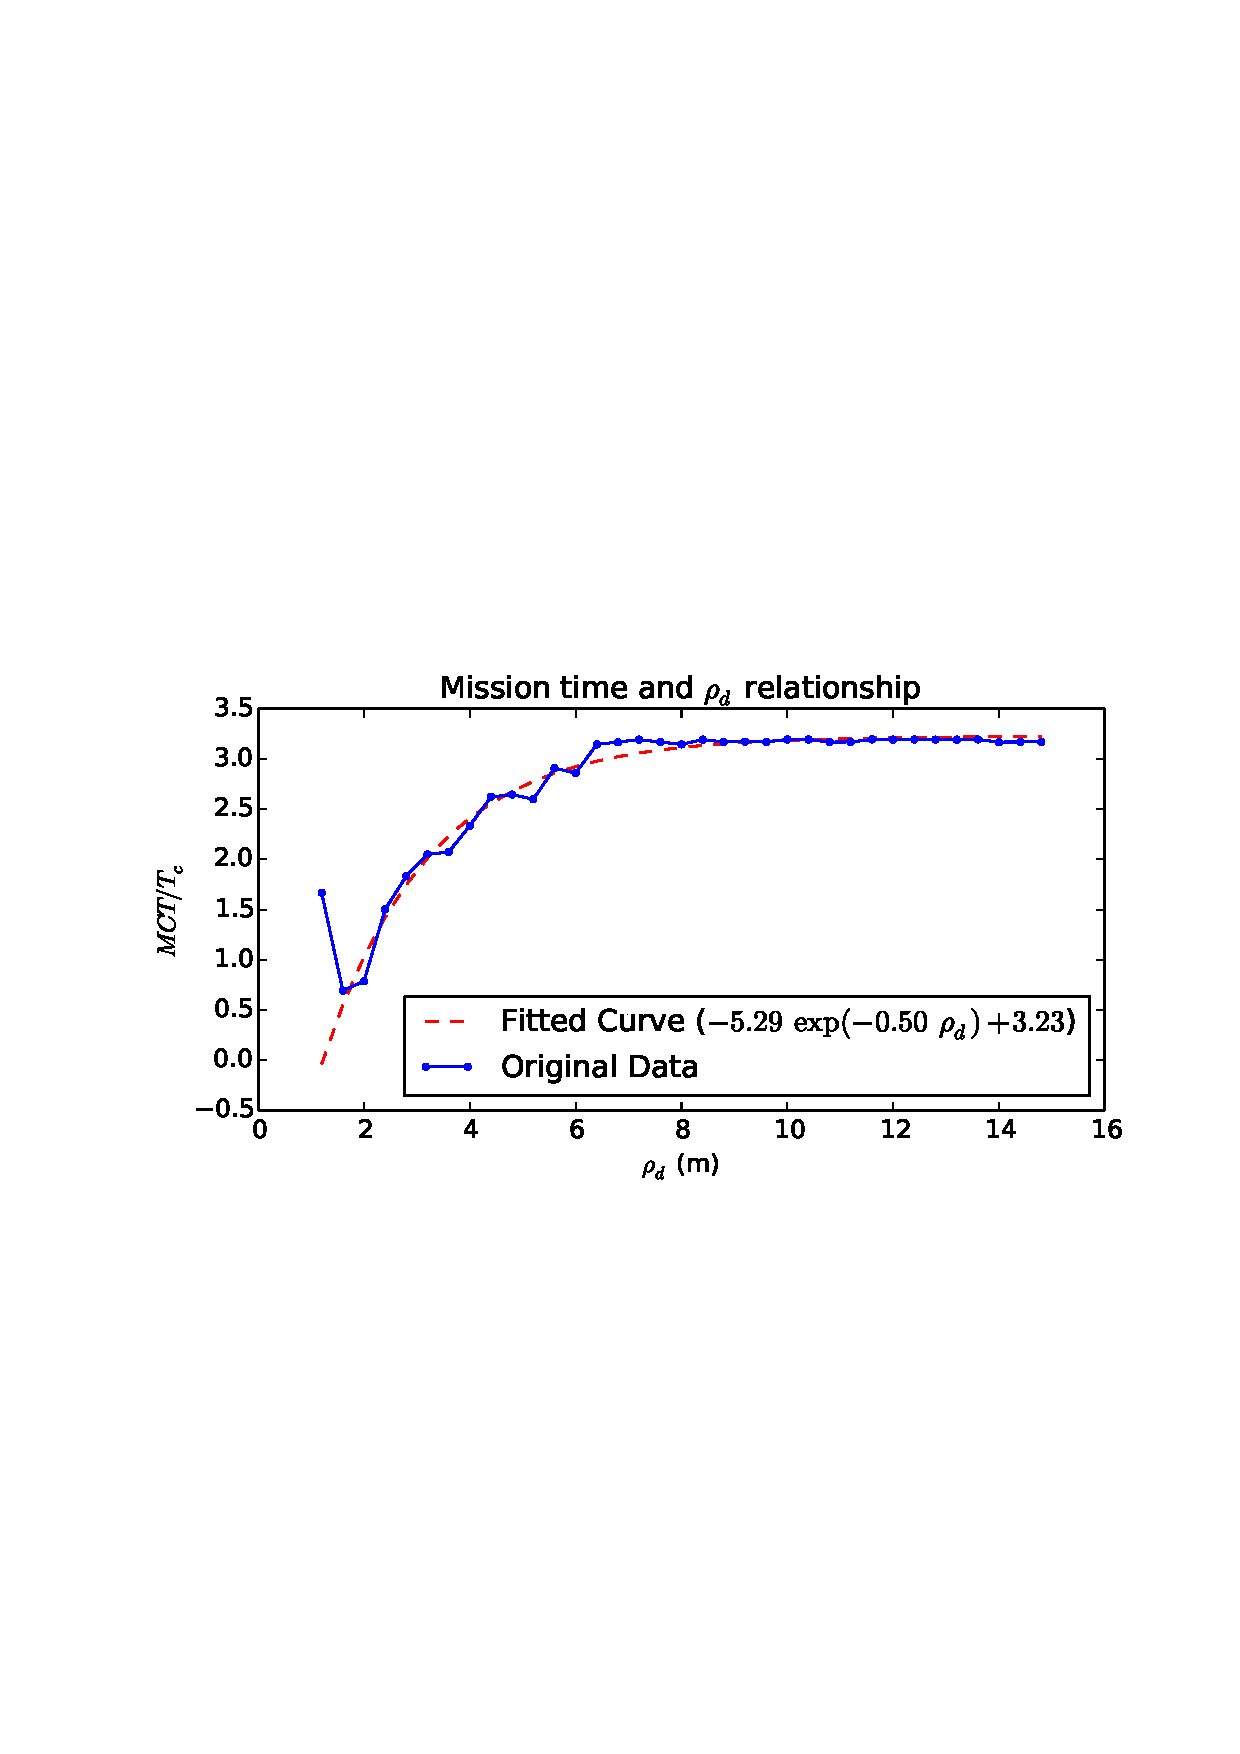
\includegraphics[width=.65\linewidth]{./images/drho/drho-rmp.pdf} % <-- use this
  %\rule{5cm}{5cm} % <-- this is just a black box substitute for graphics
  \caption{Increasing of detection radius and impact on a $MTC/T_c$ 
ratio\label{fig:drhormp}}
\end{figure}
Another parameter having direct impact on the $MCT/T_c$ ratio is the detection radius
of the robot's sensors.
As the detection radius of the robot increases, more obstacles are
seen at once which, in turn,
increases the number of constraints in the optimization problems.
The impact of increasing the detection radius $d_{sen}$ in the $MCT/T_c$ ratio can
be seen in the Figure~\ref{fig:drhormp} for a scenario with seven obstacles.
The computation time stops increasing as soon as the robot sees all obstacles present in the environment.

%\subsection{Parameters' impact analyses}

%\begin{itemize}
% \item 
% $O(N_{knots}^3)$ time is requested; 
% \item 
% $O(N_s)$ time is requested;
%\end{itemize}

\subsubsection{Obstacle penetration $P$}

Obstacle penetration area $P$ gives a metric for obstacle avoidance and 
consequently for solution quality. A solution where the planned trajectory does not pass through 
an object at any instant of time gives $P = 0$. The greater the $P$ the worse is the solution. 
However, since time sampling is performed during the optimization, $P$ is usually greater than 
zero.
A way of assuring $P = 0$ would  be to increase the obstacles radius computed by the robot's 
perception system by the 
maximum distance that the robot can run within the time spam $T_p/N_s$. However simple,
this approach represents a loss of optimality and is not considered in this work.

It is relevant then to observe the impact of the algorithm parameters in the obstacle 
penetration area.
$T_c/T_p$ ratio, $N_{knots}$ and $d_{sen}$ impact on this criteria is only 
significant for degraded cases, meaning that around typical values those parameters 
do not change $P$ significantly. However, time sampling $N_s$ is a relevant parameter.
Figure~\ref{fig:res} shows the penetration area decreasing as the number of samples 
increases.
\begin{figure}[H]\centering
  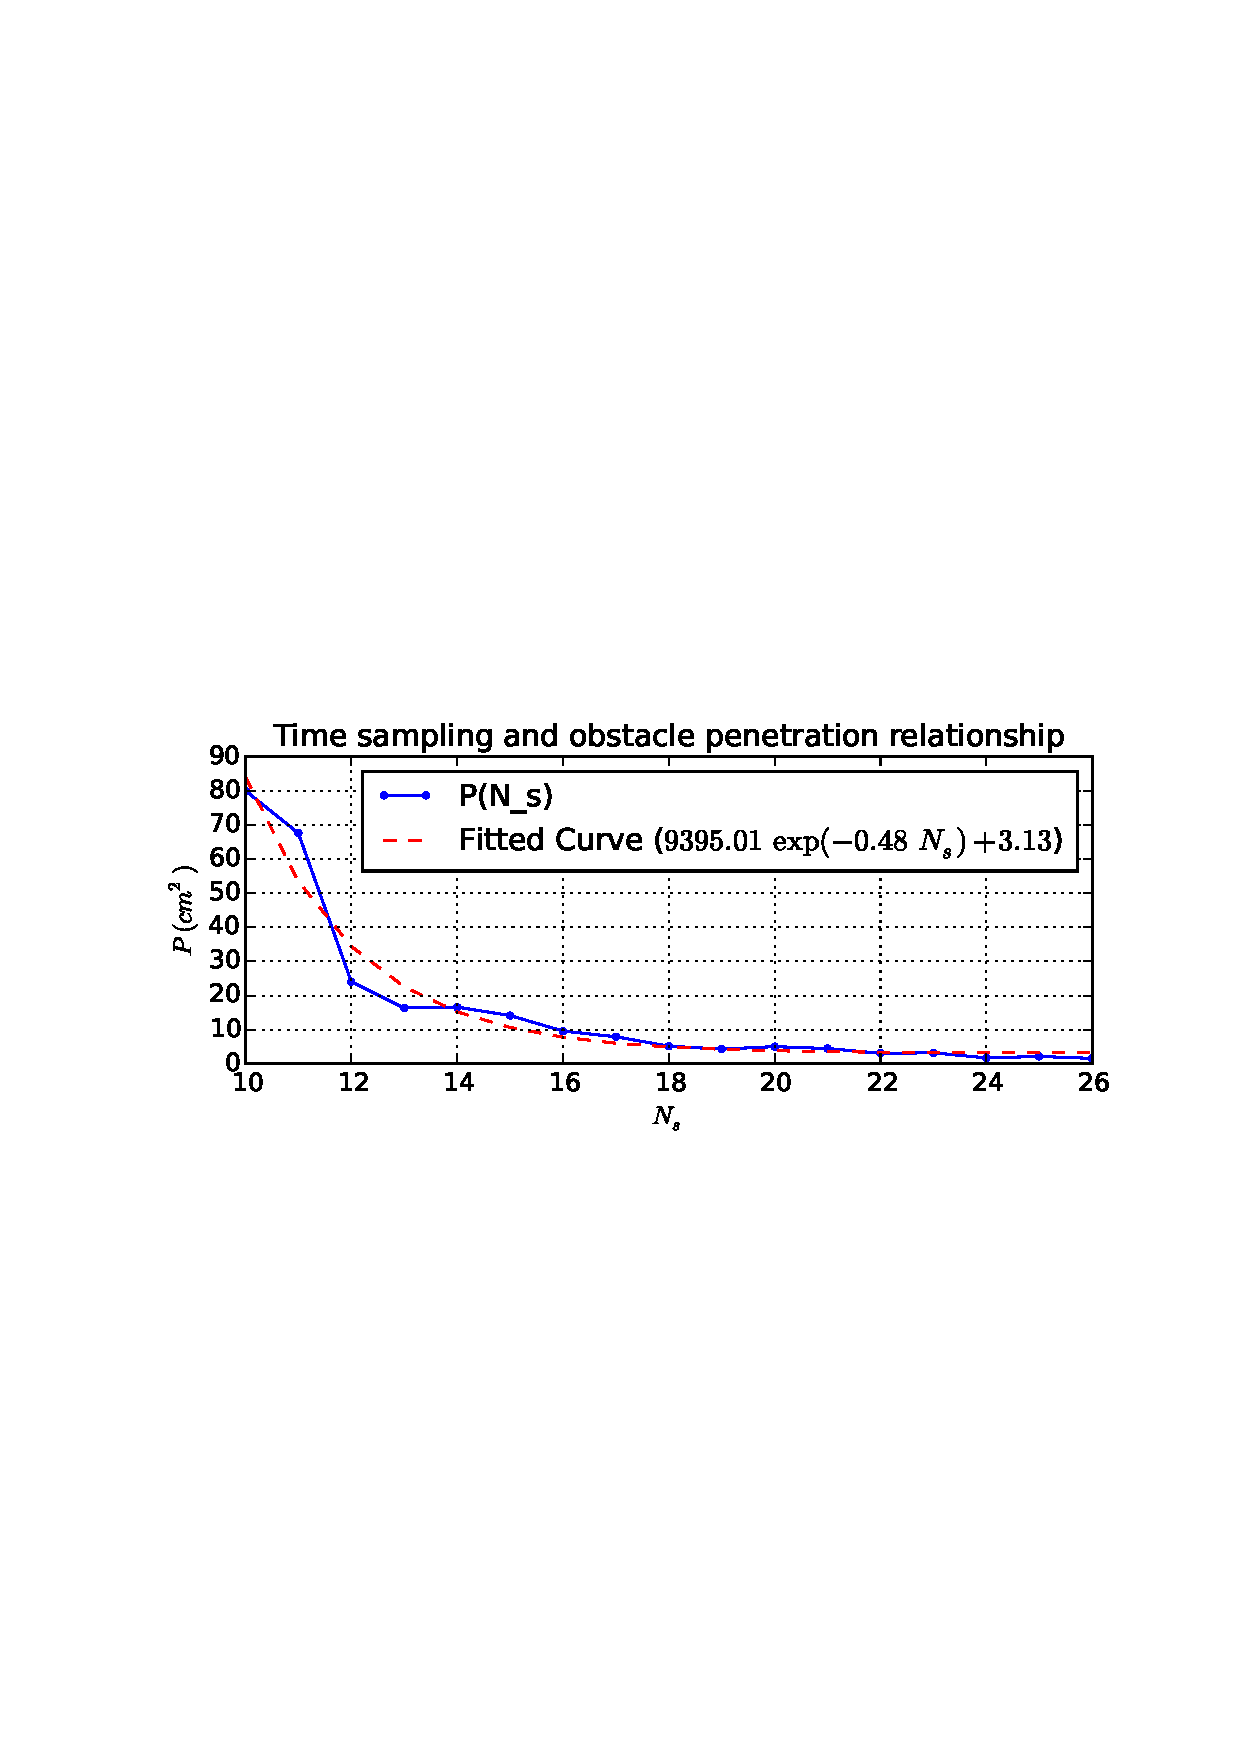
\includegraphics[width=.65\linewidth]{./images/penetration/pen-nsi.pdf} %
  %\rule{5cm}{5cm} % <-- this is just a black box substitute for graphics
  \caption{Obstacle penetration decreasing as sampling increases}
\label{fig:res}
\end{figure}
%\subsubsection{Detection radius impact}
%Ideally we would have Pw = 0. A way of guarantying that would be to increase the
%obstacles radius computed by the robot's perception system by the maximum distance that
%the robot can run within the time spam Tp /Ns (equivalent to Tc /NTc ). However simple,
%this approach represents a loss of optimality and will not be considered in this work.1
%These two behaviors indicate how a compromise between computation time and optimality must be found.
\subsubsection{Travel time $T_{tot}$}
%
Another complementary metric for characterizing solution quality is the travel time
$T_{tot}$. Analyses of data from several simulations show a tendency that for a given value 
of $N_{knots}$, $N_s$ and $T_c$ the travel time decreases as the planning horizon $T_p$ decreases.
This can be explained by the simple fact that for a given $T_c$, a more optimal solution (in terms of travel time) can be found if the planning horizon $T_p$ is smaller.
%Figure~\ref{fig:ttot} show data that supports these analysis.
%\begin{figure}[H]
%        \centering
%        ~ %add desired spacing between images, e. g. ~, \quad, \qquad, \hfill etc.
%          %(or a blank line to force the subfigure onto a new line)
%        \begin{subfigure}[b]{0.48\textwidth}
%                \includegraphics[width=\textwidth]{./images/tot/tot10.eps}
%                \caption{$N_s = 10$}\label{fig:ttot1}
%        \end{subfigure}
%        ~ %add desired spacing between images, e. g. ~, \quad, \qquad, \hfill etc.
%          %(or a blank line to force the subfigure onto a new line)
%        \begin{subfigure}[b]{0.48\textwidth}
%                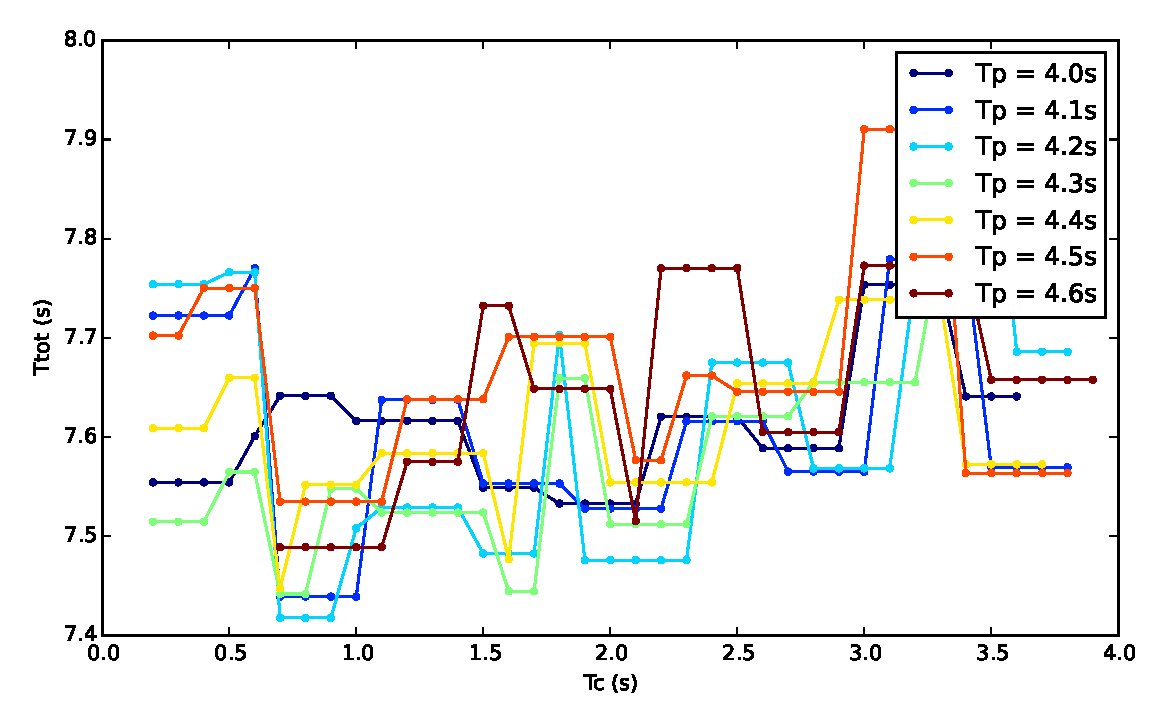
\includegraphics[width=\textwidth]{./images/tot/tot11.eps}
%                \caption{$N_s = 11$}\label{fig:ttot2}
%        \end{subfigure}
%        
%        ~ %add desired spacing between images, e. g. ~, \quad, \qquad, \hfill etc.
%          %(or a blank line to force the subfigure onto a new line)
%        \begin{subfigure}[b]{0.48\textwidth}
%                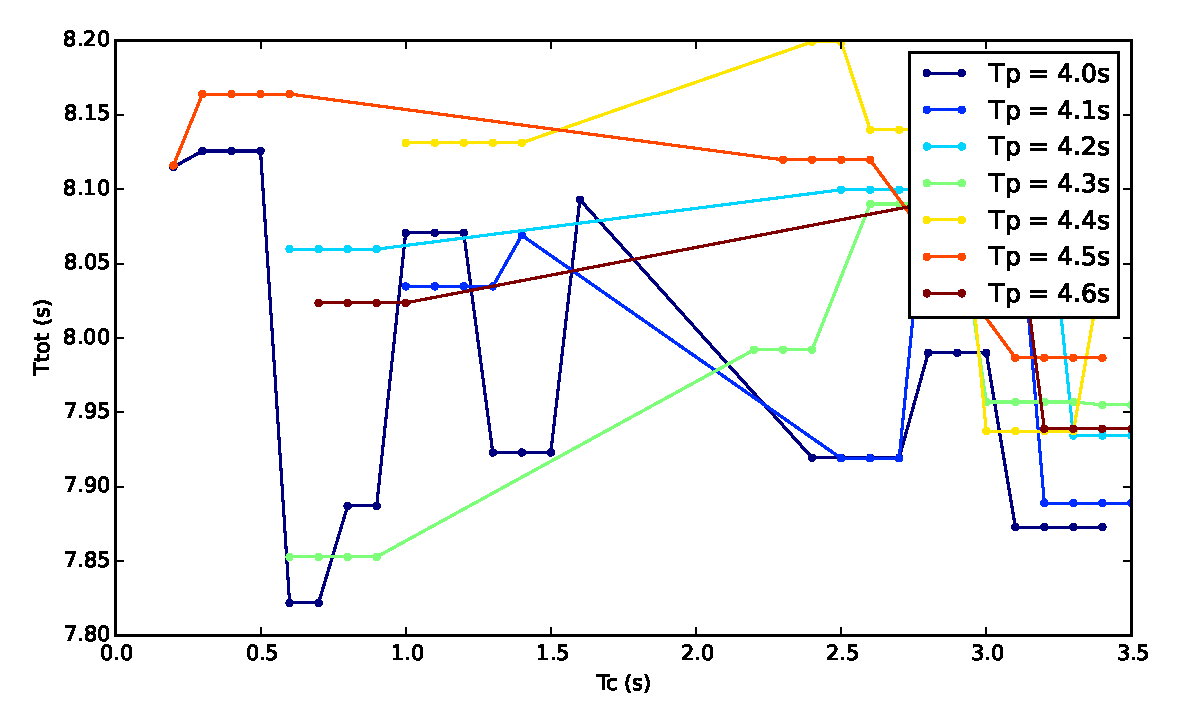
\includegraphics[width=\textwidth]{./images/tot/tot12.eps}
%                \caption{$N_s = 12$}\label{fig:ttot3}
%        \end{subfigure}
%        \caption{Variation of total travel time with the computation horizon ($T_c$) for differet planning horizons ($T_p$) and sampling number ($N_s$) in three obstacles scenarion.}\label{fig:ttot}
%\end{figure}
Another relevant observation is that the overall travel time is shorter for smaller $N_s$'s. 
This misleading improvement does take into account the fact 
that the fewer the samples the greater will be the obstacle penetration area as shown previously in Figure~\ref{fig:res}.

Furthermore, the Figure~\ref{fig:drhotot} shows travel time
invariance for changes in the detection radius far from degraded values that are too small.
This points out that a local knowledge of the environment provides enough information for finding good solutions.
\begin{figure}[H]\centering
  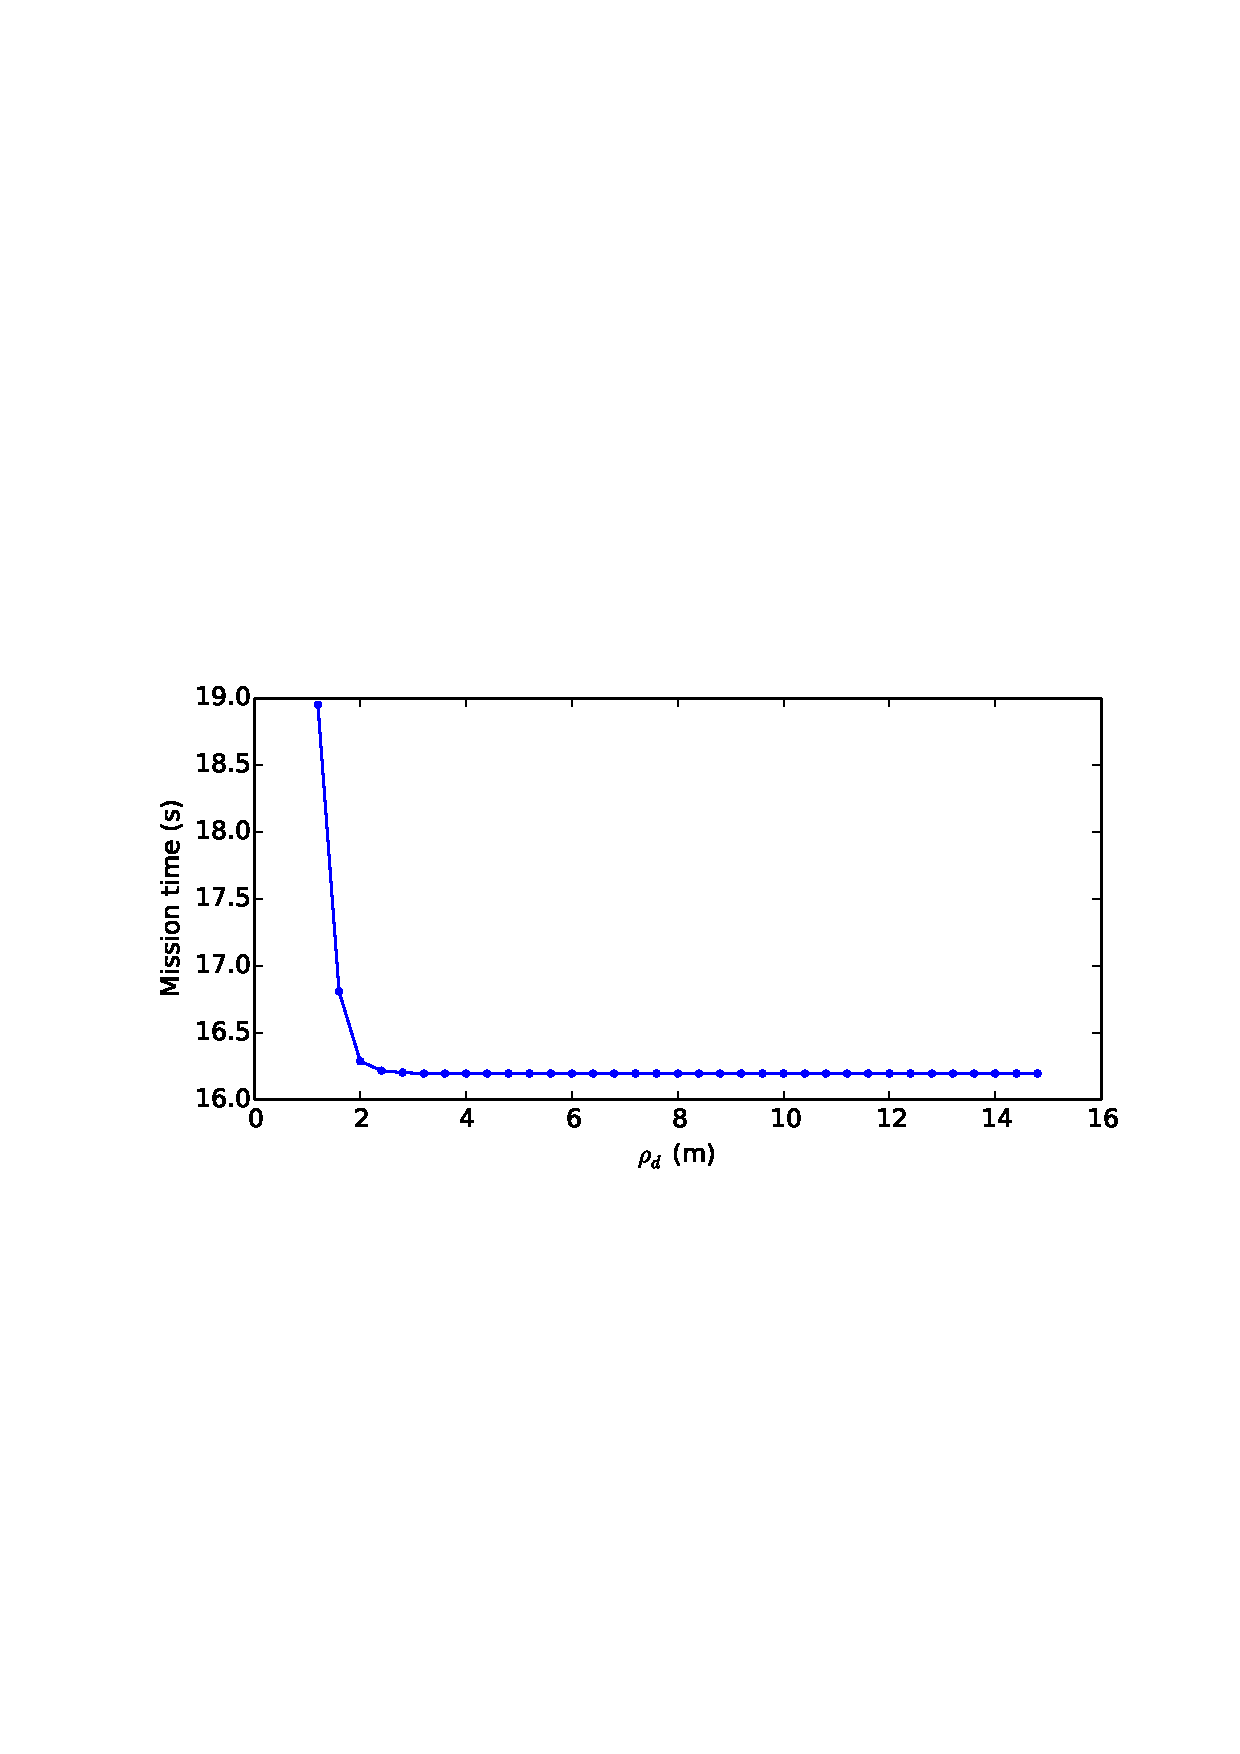
\includegraphics[width=.65\linewidth]{./images/drho/drho-tot.pdf}
  \caption{Increasing of detection radius and impact on
  $T_{tot}$\label{fig:drhotot}}
\end{figure}



\section{Tests in a dynamic simulation environment}

To test and evaluate the performance of our motion planning algorithm in a more realistic situation we used a physics simulation environment called XDE. 

XDE is a physics simulation software fully developed by CEA-LIST that can handle a variety of physical aspects such as deformable bodies, multibody systems with kinematic constraints and contacts, and fluids. Its utilization presents though some rough edges and a steep learning curve.

To use it we needed to reimplement the motion planning algorithm in C++ and interface it with XDE features.

At the beginning of the implementation of the algorithm on XDE we used the optimization library NLOPT. It supports the same solver SLSQP used before, requiring though the user to implement the computation of the objective function gradient and the constraints Jacobian matrix.

Finding those analytic derivatives is not trivial. Probably due to some error while calculating them, our fist implementation using the SLSQP solver halted after the first iteration due to round off errors.

An attempt to use the package ADOL-C for obtaining the derivatives needed  in order to use the SLSQP solver was done. We stop getting round off errors but the results using the SLSQP were still far from acceptable.

Due to a lack of time, we used then the derivative-free solver COBYLA (present also in the NLOPT package) to generate the results presented in the following.


\subsection{Results for the preliminary dynamic simulation}

%During the third month and beginning of the forth while producing the analysis referenced by the latest subsection we begin porting the implementation done in python to the XDE environment. 

%The objective is to get much closer to a real physical system being able to implement dynamic behavior in the simulated environment which was previously neglected.

An overview of the simulator visual environment showing the unicycle mobile robot used for implementing the algorithm can be seen in Figure~\ref{fig:xde}.
%For instance the obstacle detection can be based on real sensors models carrying uncertainties instead of assuming the absolute knowledge of an obstacle position as soon as it enters within the robot's detection radius.
%\clearpage
\begin{figure}[H]
	\centering
	\includegraphics[width=0.6\textwidth]{./images/xde4.png}
	\caption{XDE - unicycle mobile robot application\label{fig:xde}}
\end{figure}

Our preliminary results for this implementation for a simple scenario described in the Table~\ref{tab:xdesimin} can be seen bellow from Figure~\ref{fig:xde1} to~\ref{fig:xde3}. In red we have the solution found by the algorithm while in blue we have the simulated robot's actual path, velocities and yaw. The input generated by our motion planner were directly send to the simulated robot, no controller nor use of state feedback information were implemented.

\begin{table}[H]
\caption {Values for scenario definition} \label{tab:xdesimin}
\begin{center}
\begin{tabular}{|c|c|}
\hline
$v_{max}$ & $0.80\ \mathrm{m/s}$\\
\hline
$\omega_{max}$ & $1.80\ \mathrm{rad/s}$\\
\hline
$q_{inital}$ & $[0.00\ 0.00\ 0.00]^T$\\
\hline
$q_{final}$ & $[6.00\ 6.00\ 0.00]^T$\\
\hline
$u_{initial}$ & $[0.00\ 0.00]^T$\\
\hline
$u_{goal}$ & $[0.00\ 0.00]^T$\\
\hline
\end{tabular}
\end{center}
\end{table}

\begin{figure}[H]\centering
  \includegraphics[width=.49\textwidth]{./images/xde/PLOT_no_acc/dy_path.pdf}
  %\includegraphics[width=.48\textwidth]{./images/xde/PLOT_no_acc/ang.pdf}
  \includegraphics[width=.49\textwidth]{./images/xde/PLOT_no_acc/dy_vw.pdf}
  \caption{Comparison between planned and actual behavior for the dynamic simulation ($T_c = 0.4,\ T_p = 1.0$), no constraints on acceleration\label{fig:xde1}}
\end{figure}

\begin{figure}[H]\centering
  \includegraphics[width=.49\textwidth]{./images/xde/PLOT_acc_osc/dy_path.pdf}
  %\includegraphics[width=.48\textwidth]{./images/xde/PLOT_acc_osc/ang.pdf}
  \includegraphics[width=.49\textwidth]{./images/xde/PLOT_acc_osc/dy_vw.pdf}
  \caption{Comparison between planned and actual behavior for the dynamic simulation ($T_c = 0.4,\ T_p = 1.0$), constraints on acceleration: $|\dot{v}| \leq 0.40\ \mathrm{m/s^2},\ |\dot{\omega}| \leq 0.70\ \mathrm{rad/s^2}$\label{fig:xde2}}
\end{figure}

\begin{figure}[H]\centering
  \includegraphics[width=.49\textwidth]{./images/xde/PLOT_acc_noosc/dy_path.pdf}
  %\includegraphics[width=.48\textwidth]{./images/xde/PLOT_acc_noosc/ang.pdf}
  \includegraphics[width=.49\textwidth]{./images/xde/PLOT_acc_noosc/dy_vw.pdf}
  \caption{Comparison between planned and actual behavior for the dynamic simulation ($T_c = 0.2,\ T_p = 1.0$), constraints on acceleration: $|\dot{v}| \leq 0.40\ \mathrm{m/s^2},\ |\dot{\omega}| \leq 0.70\ \mathrm{rad/s^2}$\label{fig:xde2}}
\end{figure}

For the first of the three simulations (Figure~\ref{fig:xde1}) we can notice that dynamics effects prevents the simulated robot to follow high changes in the planned velocities. Consequently, we have very high errors in the in the planned and actual robot's configuration along the simulation. This behavior is understandable since the robot's dynamic model is neglected in the formulation of the problem.

for simulations represented in Figure~\ref{fig:xde2} and Figure~\ref{fig:xde3} we changed the set of constraints in the NLPs so angular and linear accelerations could be taken into account. We limited the module of those accelerations by arbitrary values.

Constraining the accelerations had the impact of significatively decreasing the errors in position and yaw. Two downsides of this approach for improving the generated solution with respect to dynamics effects are:

\begin{itemize}
\item [$\bullet$] Increase in the computation time. Adding accelerations constraints adds approximately $(N_s-1)*p$ inequations to each NLP.

\item [$\bullet$] Possibility of oscillation effects as the one present in Figure~\ref{fig:xde2}. Simulations represented in Figure~\ref{fig:xde2} and Figure~\ref{\ref{fig:xde3} differ only in the computation/update horizon $T_c$. $T_c$ for Figure~\ref{\ref{fig:xde3} is half of the one used in Figure~\ref{\ref{fig:xde2}.

\end{itemize}

Some implementation problems can be identified in this solution even though the scenario is very simple. For instance, violation of some constraints in the in the termination planning stage are present. We can notice that the error between the planned final configuration and the goal configuration is too high.


%Valid for SLSQP-based sovler:
%
%\begin{itemize}
% \item [$\bullet$] $MCT/T_c$ is $O(n^3)$ time dependent where $n$ is directly proportional to $N_{knots}$;
% \item [$\bullet$] $MCT/T_c$ is $O(n)$ where $n$ is directly proportional to $N_s$;
% \item [$\bullet$] $MCT/T_c$ increases as the detection radius of the robot increases;
% \item [$\bullet$] $T_{tot}$ decreases as $N_s$ decreases (up to a minimum value);
% \item [$\bullet$] $T_{tot}$ is not influenced by $T_c$ in a observable way;
% \item [$\bullet$] $T_{tot}$ decreases as the $N_{knots}$ increases (but not indefitalely);
% \item [$\bullet$] $P$ increases as $N_s$ decreases (up to a maximum value);
%\end{itemize}
%
%"Semantic" interpretation/analysis of the obstacles can speedup NPL solving by reducing the number of contraints.
%
%"Calibration" of the parameters can be done once knowing the real application conditions:
%\begin{itemize}
% \item [$\bullet$] Approx. obstacles "density";
% \item [$\bullet$] Robots max speed;
% \item [$\bullet$] Approx. distance;
% \item [$\bullet$] etc.
% \end{itemize}
%by simulating before and pay attention to the behavior of important values such as $MCT/T$, $T_{tot}$, $P$.



%TODO Comparison with the other method;
%
%TODO Before concluding do comparison with other approach and make sure to have 
%multi-robot stuff

%\chapter{Algorithmic Approach}
%\section{Distributed Motion Planning}
%\lipsum[1]
%\newpage
%
%%The optimization problem for the first implementation:
%
%% \begin{equation}
%% 	\underset{(t_{final},C_0,\dotsc,C_{d+n_{knot}-2})}{\mathrm{min}} J = \int_{t_{initial}}^{t_{final}}dt
%% \end{equation}
%
%\begin{equation}
%	\underset{(t_{final},C_0,\dotsc,C_{d+n_{knot}-2})}{\mathrm{min}} J = (t_{final}-t_{initial})^{2}
%\end{equation}
%
%under the following constraints $\forall k \in \{0,\dotsc,N_s -1\}$:
%\begin{equation}%\label{eq:sysr4}
%\left\lbrace\begin{array}{lcl}
%    \varphi_1(z(t_{initial}),\dotsc,z^{(l-1)}(t_{initial})) & = & q_{initial}\\
%    \varphi_1(z(t_{final}),\dotsc,z^{(l-1)}(t_{final})) & = & q_{final}\\
%    \varphi_2(z(t_{initial}),\dotsc,z^{(l)}(t_{initial})) & = & u_{initial}\\
%    \varphi_2(z(t_{final}),\dotsc,z^{(l)}(t_{final}))& = & u_{final}\\
%    \varphi_2(z(t_k),\dotsc,z^{(l)}(t_k)) &\in& \mathcal{U}\\
%    d_{O_m}(t_k) &\geq& \rho + r_m,\quad \forall O_m \in \mathcal{Q}_{occupied}
%\end{array}\right.
%\end{equation}

% \paragraph{Practical stuff for implementation}
% 
% $q \in \R^n$ and $u \in \R^m$. $N_s$ number of time steps used when computing the problem.
% 
% Number of equations: $2n + 2m$
% 
% Number of inequations: $N_s(m+\mathrm{card}(\mathcal{Q}_{occupied}))$

% \paragraph{OPTIMIZERS}\footnote{CFSQP, SNOPT, NLPQL and FSQP are licensed} CFSQP is the name of the solver used by Defoort.

% \paragraph{SCIPY} Constrained minimization

% "Method L-BFGS-B uses the L-BFGS-B algorithm [R106], [R107] for bound constrained minimization.

% Method TNC uses a truncated Newton algorithm [R105], [R108] to minimize a function with variables subject to bounds. This algorithm uses gradient information; it is also called Newton Conjugate-Gradient. It differs from the Newton-CG method described above as it wraps a C implementation and allows each variable to be given upper and lower bounds.

% Method COBYLA uses the Constrained Optimization BY Linear Approximation (COBYLA) method [R109], [10], [11]. The algorithm is based on linear approximations to the objective function and each constraint. The method wraps a FORTRAN implementation of the algorithm.

% Method SLSQP uses Sequential Least SQuares Programming to minimize a function of several variables with any combination of bounds, equality and inequality constraints. The method wraps the SLSQP Optimization subroutine originally implemented by Dieter Kraft [12]. Note that the wrapper handles infinite values in bounds by converting them into large floating values."

% \paragraph{PYOPT}
% "We can see that for this convex problem, the four SQP optimizers (SNOPT, NLPQL, SLSQP, and FSQP) provide the most accurate solutions for the specified convergence tolerance. The FSQP optimizer requires the largest number of evaluations of all SQP approaches, since it generates a feasible point at each iteration before solving the SQP subproblem."

% There are other two optimizers that work: PSQP ALGENCAN

%\begin{itemize}
%\item Problem with discretization
%
%Try adding CONSTRAINTS related to max acceleration (\textcolor{red}{DONE})
%
%For that we have to increase the maximum derivative order of the flat output needed so we calculate $[\dot{v}\ \dot{\omega}]$ building a $\varphi_3$ function
%
%Also, the constraints to be added:
%\[
%	\varphi_3(z(t_k),\dotsc,z^{(l)}(t_k)) \in \mathcal{A}
%\]
%where $\mathcal{A}$ is the set of admissible acceleration values.
%
%The function $\varphi_3$ is as follows:
%\[
%\begin{array}{l}
%\varphi_3(z(t_k),\dotsc,z^{(3)}(t_k))=\\
%=\left[\begin{array}{c}
%\dot{v}\\
%\dot{\omega}
%\end{array}\right]
%= \left[\begin{array}{c}
%\frac{\partial}{\partial t}\|\dot{z}\|\\
%\frac{\partial}{\partial t}\frac{(\dot{z}_1\ddot{z}_2-\dot{z}_2\ddot{z}_1)}{\|\dot{z}\|^2}
%\end{array}\right] = \left[\begin{array}{c}
%\frac{\dot{z}_1\ddot{z}_1 + \dot{z}_2\ddot{z}_2}{\|\dot{z}\|}\\
%\frac{(\ddot{z}_1\ddot{z}_2+ z^{(3)}_2\dot{z}_1 - (\ddot{z}_2\ddot{z}_1+z^{(3)}_1\dot{z}_2))\|\dot{z}\|^2-2(\dot{z}_1\ddot{z}_2-\dot{z}_2\ddot{z}_1)\|\dot{z}\|\dot{v}}{\|\dot{z}\|^4}
%\end{array}\right]
%\end{array}
%\]

% \item Error over max value
% \item change ACC according to the max speed

% Kludge to reach convergence was decreasing accuracy (increasing the value of the ACC option).
% 
% ACC equals to $0.5e-2$ works but seems really bad since the default value used on all algorithms based on the Dieter Kraft implementation in FORTRAN use $1e-6$.
% 
% In my opinion, this suggests an error on my optimization problem definition or it could be the simple fact that with so many constraints (over 700 constraints) it is hard to a have a high accuracy "at the same time"

%\item Remake code using good objected oriented structure. It will be good for C++ part (\textcolor{red}{DONE})
%
%\end{itemize}

% \includegraphics[width=0.5\textwidth]{./img/planning-sim-trajc.png}

% \includegraphics[width=0.5\textwidth]{./img/planning-sim-trajc-good.png}

% \includegraphics[width=0.5\textwidth]{./img/planning-sim-vw-good.png}

%\paragraph{ONLINE}
%
%$T_c$ and $T_p$ (planning horizon) "given" (arbitrary).
%
%\[
%	\tau_{k} = t_{initial}+kT_c\quad k \in \N
%\]
%
%Arbitrary detection radius for the robot sensors. Only if the obstacle characteristic position  is inside the detection zone the obstacle is considered detected. Using $2m$.
%
%Evaluate for each time interval $[\tau_{k-1},\tau_k) (k \in \N)$ the trajectory beginning at $\tau_k$ until $\tau_k+T_p$:
%
%\begin{equation}
%	\underset{(C_{(0,\tau_k)},\dotsc,C_{(d+n_{knot}-2,\tau_k)})}{\mathrm{min}} J_{\tau_k} = \|\varphi_1(z(\tau_k+T_p,\tau_k),\dotsc,z^{(l-1)}(\tau_k+T_p,\tau_k))-q_{final}\|^2
%\end{equation}
%
%under the following constraints $\forall t \in [\tau_k, \tau_k+T_p]$:
%\begin{equation}%\label{eq:sysr4}
%\left\lbrace\begin{array}{lcl}
%	\varphi_1(z(\tau_{k},\tau_{k}),\dotsc,z^{(l-1)}(\tau_k,\tau_k)) & = & q_{ref}(\tau_k,\tau_{k-1})\\
%    \varphi_2(z(\tau_{k},\tau_{k}),\dotsc,z^{(l)}(\tau_k,\tau_k)) & = & u_{ref}(\tau_k,\tau_{k-1})\\
%    \varphi_2(z(t,\tau_k),\dotsc,z^{(l)}(t,\tau_k)) &\in& \mathcal{U}\\
%    d_{O_m}(t,\tau_k) &\geq& \rho + r_m,\quad \forall O_m \in \mathcal{O}(\tau_k)
%\end{array}\right.
%\end{equation}
%
%The period $[\tau_{-1},\tau_0)$ is what is called by Defoort "the initialization phase" which considers: $$q_{ref}(\tau_0,\tau_{-1}) = q_{initial}$$ $$u_{ref}(\tau_0,\tau_{-1}) = u_{initial}$$ without no more further changes to the expressions above.


%\paragraph{Practical stuff for implementation}
%
%$q \in \R^n$ and $u \in \R^m$. $N_s$ number of time steps used when computing the problem.
%
%Number of equations: $n + m$
%
%Number of inequations (function of $\tau_k$): $N_s(m+\mathrm{card}(\mathcal{O}(\tau_k)))$
%
%dependencies:
%sudo apt-get install python python-dev libatlas-base-dev gcc gfortran g++
%
%get source:
%https://pypi.python.org/pypi/scipy
%
%sudo python setup.py install
%
%\section{The mobile robot}
%
%For representing the mobile robot geometry in the planning plane a bounding circle was chosen.
%
%\subsection{Unicycle kinetic model}
%
%\subsection{Flat output formulation}
%\pagebreak



%\begin{figure}[H]
%	\centering
%	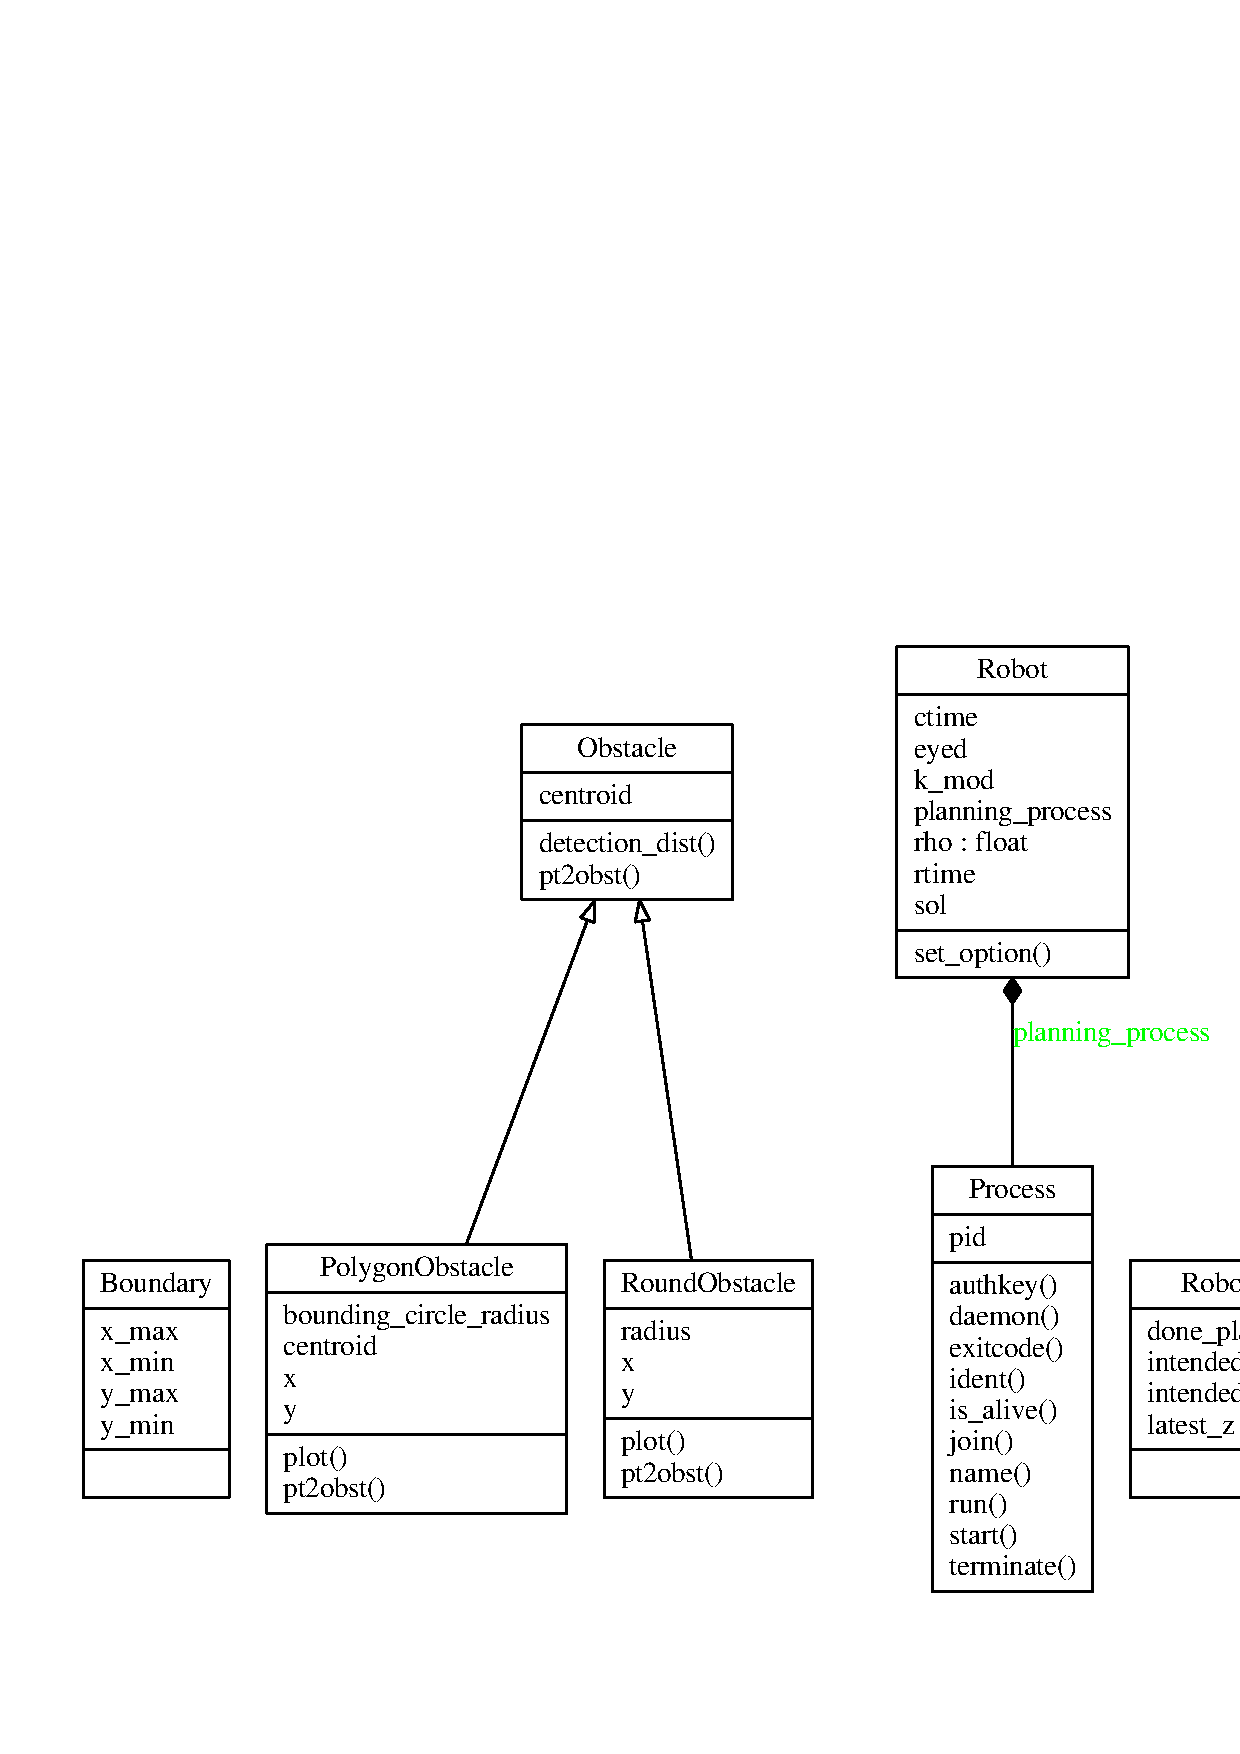
\includegraphics[width=1.\textwidth]{./img/classes_planning.pdf}
%	\caption{Class diagram.\label{fig:classesdiagram}}
%\end{figure}
%\subsection{Analysis of real-time planning feasibility}
%\subsection{Multi-robots}
%Each robot must be able to access the position of any robot of the fleet. If a robot's position cannot be accessed that means the robot lost its connection with the fleet and will not be considered a conflictual robot by none of the others robots.
%Symmetry problem \todo[inline, size=\tiny]{Tc too high no time to avoid another robot involved}
%Gilbert-Johnson-Keerthi distance algorithm

%\section{Analysis of the parameters impact on real-time feasibility and solution adequacy}
%
%The performance and solution quality of the motion planning algorithm previously presented depends on several parameters.
%These parameters can be split into two groups. The \textbf{algorithm related} parameters and the \textbf{optimization solver related} ones.
%Among the former group, the most important ones are:
%\begin{itemize}
%\item[$\bullet$] The number of sample for time discretization ($N_s$);
%\item[$\bullet$] The number of internal knots for the B-splines curves ($n_{knots}$);
%\item[$\bullet$] The planning horizon for the sliding window ($T_p$);
%\item[$\bullet$] The computation horizon ($T_c$).
%\end{itemize}
%
%The latter kind depends on the optimization solver adopted. However, since most of them are iterative methods, it is common to have at least the two following parameters:
%\begin{itemize}
%\item[$\bullet$] Maximum number of iterations;
%\item[$\bullet$] Stop condition.
%\end{itemize}
%
%%The task of searching for a satisfactory set of parameters' values with regard to a performance metric (e.g. total time to complete the miss1ion) is quite laborious.
%
%This high number of parameters having influence on the solution and/or on the time for finding a solution makes the search for a satisfactory set of parameters' values a laborious task.
%
%We attempt nevertheless to extract some quantitative knowledge about how these parameters impact the generated solution and its computation time based on several simulations run with different parameters configurations.
%The main objective here is to be able to support the feasibility of a real-time motion planner based on this algorithm.
%
%After these analyses we shall be able to identify sets of parameters' values that minimize the total time spend to complete the mission, respecting the problem constraints
%and minimizing the \textit{maximum computation time}/$T_c$ ratio.
%
%\subsection{Computation time analysis}
%
%At first we were interest in finding how variations in $N_s$ and $N_{knots}$ impart the computation time for finding a solution.
%
%Aiming for a scenario invariant understanding of the impact of these parameters three different scenarios were studied. A first scenario where the robot did not had to avoid any obstacle
%to complete its mission, a second one where three round obstacles were randomly generated in a region where the robot was probably going to pass through and a third similar to the second
%only with six instead of three obstacles.
%
%In addition, to reduce the problem's size, a unique optimization solver with fixed parameters was used for all simulations.
%The used parameters can be seen in table~\ref{tab:optparam}. The subscribed words \textit{first}, \textit{inter} and \textit{last} indicate that the respective maximum numbers of iteration are used for the first
%optimization problem solving, for all intermediaries ones and for the last one.
%Different maximum numbers of iterations are used for different stages of the planning process. This is possible because of two aspects of the problem addressed:
%\begin{itemize}
%\item[$\bullet$] We assume that the initial configuration at time $t_0$ is static and thus the planning of the first section of the plan does not have to be done within the computation horizon ($T_c$). We choose then to increase the maximum number of iterations for the first planning section in order to achieve better results;
%\item[$\bullet$] According to the change in the algorithm for solving the NPL associated with the last section of the plan we know that the last step uses a number of internal knots
%($N_{knots}$) smaller than or equal to the number used by the other steps. In the other hand, this final NPL has more constraints than the others NPLs solved before for a given $N_s$.
%Since the SLSPQ method requires $O(n^3)$ time to find a solution, where $n$, the dimension of the parameter vector, is directly proportional to the number of internal knots we assume
%that the number of maximum iterations for the last step can be increased.
%
%%The NPL solved for last planning section has more constraints then the others NPLs. This alone does not justify giving it a greater maximum number of iterations since the solution still must be found within a $T_c$ horizon. The other factor that allow us to decrease it is that 
%\end{itemize}
%
%%\todo[inline]{talk about accuracy}
%
%\begin{table}[H]
%\caption {Optimization solver parameters} \label{tab:optparam}
%\begin{center}
%\begin{tabular}{|c|c|}
%\hline
%Optimization solver type & SLSQP\\
%\hline
%$MAXIT_{first}$ & 40\\
%\hline
%$MAXIT_{inter}$ & 15\\
%\hline
%$MAXIT_{last}$ & 20\\
%\hline
%accuracy & $10^{-3}$\\
%\hline
%\end{tabular}
%\end{center}
%\end{table}
%
%Real-time feasibility in this context can be considered as having the \textit{maximum computation time} spend for planning the path sections
%\footnote{All computational times spend for planning all sections are considered for finding the maximum value but the first one} less than or equal to the computation horizon ($T_c$).
%Here though we are only interest in understanding the variation of \textit{maximum computation time}/$T_c$ with changes in $N_s$ and $N_{knots}$.

%Another natural performance metric that should be kept in mind is the total time spend to complete the mission (going from the initial configuration to the final).

%\subsubsection{No obstacles scenario}
%%INFO:R0: TOT: 7.16220241525
%%INFO:R0: NSE: 14
%%INFO:R0: FIR: 0.888309001923
%%INFO:R0: LAS: 0.311777114868
%%INFO:R0: LMA: 1
%%INFO:R0: MAX: 0.0503461360931
%%INFO:R0: MIN: 0.0204219818115
%%INFO:R0: AVG: 0.0319990317027
%%INFO:R0: RMP: 0.125865340233
%%INFO:R0: RMG: 0.77944278717
%
%The images in the Figure~\ref{fig:uni0} try to make prominent the effect of changes in the in the number of samples ($N_s$) and number of internal knots ($N_{knots}$). In the ordinate axis we have the \textit{maximum computation time}/$T_c$ ratio and in the abscissa we have the $T_c/T_p$. For each $N_s$ we took the average of the \textit{maximum computation time}/$T_c$ ratio for a give $T_c/T_p$ among different $T_p$ values in order to be $T_p$ invariant.
%
%We can see that for a "no obstacles" scenario the overall performance with respect to the \textit{maximum computation time}/$T_c$ ratio is only slightly impacted by
%variations in the number of samples ($N_s$) and in the number of internal knots ($N_{knots}$).
%Within a given image the lines are close together showing that variations in $N_s$ have weak impact.
%In addition, comparing the three images (\ref{fig:uni04}, \ref{fig:uni05}, \ref{fig:uni06}) we see that variations in the $N_{knots}$ have also a weak influence for this scenario.
%
%\begin{figure}[H]
%        \centering
%        \begin{subfigure}[b]{0.48\textwidth}
%                \includegraphics[width=\textwidth]{./img/realtime/Scenario_0__N_knots_4/mcttc-tctp.eps}
%                \caption{Four internal knots. Average variance between lines is $0.062\times 10^{-2}$}\label{fig:uni04}
%        \end{subfigure}%
%        ~ %add desired spacing between images, e. g. ~, \quad, \qquad, \hfill etc.
%          %(or a blank line to force the subfigure onto a new line)
%        \begin{subfigure}[b]{0.48\textwidth}
%                \includegraphics[width=\textwidth]{./img/realtime/Scenario_0__N_knots_5/mcttc-tctp.eps}
%                \caption{Five internal knots. Average variance between lines is $0.115\times 10^{-2}$}\label{fig:uni05}
%        \end{subfigure}%
%        
%        ~ %add desired spacing between images, e. g. ~, \quad, \qquad, \hfill etc.
%          %(or a blank line to force the subfigure onto a new line)
%        \begin{subfigure}[b]{0.48\textwidth}
%                \includegraphics[width=\textwidth]{./img/realtime/Scenario_0__N_knots_6/mcttc-tctp.eps}
%                \caption{Six internal knots. Average variance between lines is $ 0.182\times 10^{-2}$}\label{fig:uni06}
%        \end{subfigure}%
%        \caption{Zero obstacles scenario.}\label{fig:uni0}
%\end{figure}
%
%For the sake of an example we present a simulation result in the Figure~\ref{fig:sim0} run with the parameters presented in the table~\ref{tab:s0param} for a "no obstacles" scenario.
%
%\begin{table}[H]
%\caption {Motion planner main parameters} \label{tab:s0param}
%\begin{center}
%\begin{tabular}{|c|c|}
%\hline
%$T_p$ & 2.00 s\\
%\hline 
%$T_c$ & 0.40 s\\
%\hline 
%$N_s$ & 9\\
%\hline 
%$N_{knots}$ & 5\\
%\hline
%$v_{max}$ & $1.00\ \mathrm{m/s}$\\
%\hline
%$\omega_{max}$ & $5.00\ \mathrm{rad/s}$\\
%\hline
%$q_{inital}$ & $[-0.05\ 0.00\ \pi/2]^T$\\
%\hline
%$q_{final}$ & $[0.10\ 7.00\ \pi/2]^T$\\
%\hline
%$u_{final}$ & $[0.00\ 0.00]^T$\\
%\hline
%$u_{final}$ & $[0.00\ 0.00]^T$\\
%\hline
%\end{tabular}
%\end{center}
%\end{table}
%
%\begin{figure}[H]
%        \centering
%        ~ %add desired spacing between images, e. g. ~, \quad, \qquad, \hfill etc.
%          %(or a blank line to force the subfigure onto a new line)
%        \begin{subfigure}[b]{0.48\textwidth}
%                \includegraphics[width=\textwidth]{./img/realtime/sim_results/p_0_0.4_2.0_9_5_0.001_15_40_20_5.0_0.1_3.0_0.5_1.0_10.0/multirobot-path.png}
%                \caption{Robot's path.}\label{fig:sim0rpath}
%        \end{subfigure}
%        ~ %add desired spacing between images, e. g. ~, \quad, \qquad, \hfill etc.
%          %(or a blank line to force the subfigure onto a new line)
%        \begin{subfigure}[b]{0.48\textwidth}
%		\includegraphics[width=\textwidth]{./img/realtime/sim_results/p_0_0.4_2.0_9_5_0.001_15_40_20_5.0_0.1_3.0_0.5_1.0_10.0/multirobot-vw.png}
%                \caption{Robot's input.}\label{fig:sim0rinput}
%        \end{subfigure}
%        \caption{No obstacle scenario simulation example where the \textit{maximum computation time} was about 78\% of $T_c$ and the mission total time equals to $7.16\ s$.}\label{fig:sim0}
%\end{figure}
%\clearpage
%\subsubsection{Three obstacles scenario}
%%INFO:R0: TOT: 7.57429378065
%%INFO:R0: NSE: 15
%%INFO:R0: FIR: 1.07032418251
%%INFO:R0: LAS: 0.402824163437
%%INFO:R0: LMA: 1
%%INFO:R0: MAX: 0.243094921112
%%INFO:R0: MIN: 0.0298509597778
%%INFO:R0: AVG: 0.156346522845
%%INFO:R0: RMP: 0.506447752317
%%INFO:R0: RMG: 0.83921700716
%%p_3_0.48_2.4_11_4_0.001_15_40_20_5.0_0.1_3.0_0.5_1.0_10.0
%
%For this new scenario, a greater impact of the number of samples ($N_s$) and number of non-null internal knots ($N_{knots}$) is observed.
%The greater the $N_{knots}$ or the $N_s$ the greater is the \textit{maximum computation time}/$T_c$.
%This behavior is the one expected since the number of constraints and the number of arguments for the cost function
%to be minimized depend on these two parameters respectively.
%
%\begin{figure}[H]
%        \centering
%        ~ %add desired spacing between images, e. g. ~, \quad, \qquad, \hfill etc.
%          %(or a blank line to force the subfigure onto a new line)
%        \begin{subfigure}[b]{0.48\textwidth}
%                \includegraphics[width=\textwidth]{./img/realtime/Scenario_3__N_knots_4/mcttc-tctp.eps}
%                \caption{Four internal knots. Average variance between lines is $1.047\times 10^{-2}$}\label{fig:uni34}
%        \end{subfigure}
%        
%        ~ %add desired spacing between images, e. g. ~, \quad, \qquad, \hfill etc.
%          %(or a blank line to force the subfigure onto a new line)
%        \begin{subfigure}[b]{0.48\textwidth}
%                \includegraphics[width=\textwidth]{./img/realtime/Scenario_3__N_knots_5/mcttc-tctp.eps}
%                \caption{Five internal knots. Average variance between lines is $0.972\times 10^{-2}$}\label{fig:uni35}
%        \end{subfigure}
%        ~ %add desired spacing between images, e. g. ~, \quad, \qquad, \hfill etc.
%          %(or a blank line to force the subfigure onto a new line)
%        \begin{subfigure}[b]{0.48\textwidth}
%                \includegraphics[width=\textwidth]{./img/realtime/Scenario_3__N_knots_6/mcttc-tctp.eps}
%                \caption{Six internal knots. Average variance between lines is $0.587\times 10^{-2}$}\label{fig:uni36}
%        \end{subfigure}
%        \caption{Three obstacles scenario.}\label{fig:uni3}
%\end{figure}
%
%Again, in the Figure~\ref{fig:sim0} we show a simulation example run with the parameters' values presented in table~\ref{tab:s3param}.
%
%\begin{table}[H]
%\caption {Motion planner main parameters} \label{tab:s3param}
%\begin{center}
%\begin{tabular}{|c|c|}
%\hline
%$T_p$ & 2.40 s\\
%\hline 
%$T_c$ & 0.48 s\\
%\hline 
%$N_s$ & 11\\
%\hline 
%$N_{knots}$ & 4\\
%\hline
%$v_{max}$ & $1.00\ \mathrm{m/s}$\\
%\hline
%$\omega_{max}$ & $5.00\ \mathrm{rad/s}$\\
%\hline
%$q_{inital}$ & $[-0.05\ 0.00\ \pi/2]^T$\\
%\hline
%$q_{final}$ & $[0.10\ 7.00\ \pi/2]^T$\\
%\hline
%$u_{final}$ & $[0.00\ 0.00]^T$\\
%\hline
%$u_{final}$ & $[0.00\ 0.00]^T$\\
%\hline
%$O_0$ & $[0.55\ 1.91\ 0.31]$\\
%\hline
%$O_1$ & $[-0.08\ 3.65\ 0.32]$\\
%\hline
%$O_2$ & $[0.38\ 4.65\ 0.16]$\\
%\hline
%\end{tabular}
%\end{center}
%\end{table}
%
%\begin{figure}[H]
%        \centering
%        ~ %add desired spacing between images, e. g. ~, \quad, \qquad, \hfill etc.
%          %(or a blank line to force the subfigure onto a new line)
%        \begin{subfigure}[b]{0.48\textwidth}
%                \includegraphics[width=\textwidth]{./img/realtime/sim_results/p_3_0.48_2.4_11_4_0.001_15_40_20_5.0_0.1_3.0_0.5_1.0_10.0/multirobot-path.png}
%                \caption{Robot's path.}\label{fig:rpath}
%        \end{subfigure}
%        ~ %add desired spacing between images, e. g. ~, \quad, \qquad, \hfill etc.
%          %(or a blank line to force the subfigure onto a new line)
%        \begin{subfigure}[b]{0.48\textwidth}
%		\includegraphics[width=\textwidth]{./img/realtime/sim_results/p_3_0.48_2.4_11_4_0.001_15_40_20_5.0_0.1_3.0_0.5_1.0_10.0/multirobot-vw.png}
%                \caption{Robot's input.}\label{fig:rinput}
%        \end{subfigure}
%        \caption{Three obstacle scenario simulation example where the \textit{maximum computation time} was about 84\% of $T_c$ and the mission total time equals to $7.57\ s$.}\label{fig:uni3}
%\end{figure}
%\clearpage
%\subsubsection{Six obstacles scenario}
%
%%INFO:R0: TOT: 7.76460065867
%%INFO:R0: NSE: 7
%%INFO:R0: FIR: 2.3883190155
%%INFO:R0: LAS: 0.536874055862
%%INFO:R0: LMA: 0
%%INFO:R0: MAX: 1.1533639431
%%INFO:R0: MIN: 0.116408824921
%%INFO:R0: AVG: 0.802022314072
%%INFO:R0: RMP: 0.901065580547
%%INFO:R0: RMG: 0.901065580547
%
%As for the scenario with six obstacles we realize that the observations for the latest scenario are accentuated.
%
%\begin{figure}[H]
%        \centering
%        ~ %add desired spacing between images, e. g. ~, \quad, \qquad, \hfill etc.
%          %(or a blank line to force the subfigure onto a new line)
%        \begin{subfigure}[b]{0.48\textwidth}
%                \includegraphics[width=\textwidth]{./img/realtime/Scenario_6__N_knots_4/mcttc-tctp.eps}
%                \caption{Four internal knots.  Average variance between lines is $2.272\times 10^{-2}$}\label{fig:uni64}
%        \end{subfigure}
%        ~ %add desired spacing between images, e. g. ~, \quad, \qquad, \hfill etc.
%          %(or a blank line to force the subfigure onto a new line)
%        \begin{subfigure}[b]{0.48\textwidth}
%                \includegraphics[width=\textwidth]{./img/realtime/Scenario_6__N_knots_5/mcttc-tctp.eps}
%                \caption{Five internal knots.  Average variance between lines is $2.635\times 10^{-2}$}\label{fig:uni65}
%        \end{subfigure}
%        
%        ~ %add desired spacing between images, e. g. ~, \quad, \qquad, \hfill etc.
%          %(or a blank line to force the subfigure onto a new line)
%        \begin{subfigure}[b]{0.48\textwidth}
%                \includegraphics[width=\textwidth]{./img/realtime/Scenario_6__N_knots_6/mcttc-tctp.eps}
%                \caption{Six internal knots.  Average variance between lines is $1.526\times 10^{-2}$}\label{fig:uni66}
%        \end{subfigure}
%        \caption{Six obstacles scenario.}\label{fig:uni6}
%\end{figure}
%
%
%\begin{table}[H]
%\caption {Motion planner main parameters} \label{tab:s3param}
%\begin{center}
%\begin{tabular}{|c|c|}
%\hline
%$T_p$ & 3.20 s\\
%\hline 
%$T_c$ & 1.28 s\\
%\hline 
%$N_s$ & 12\\
%\hline 
%$N_{knots}$ & 6\\
%\hline
%$v_{max}$ & $1.00\ \mathrm{m/s}$\\
%\hline
%$\omega_{max}$ & $5.00\ \mathrm{rad/s}$\\
%\hline
%$q_{inital}$ & $[-0.05\ 0.00\ \pi/2]^T$\\
%\hline
%$q_{final}$ & $[0.10\ 7.00\ \pi/2]^T$\\
%\hline
%$u_{final}$ & $[0.00\ 0.00]^T$\\
%\hline
%$u_{final}$ & $[0.00\ 0.00]^T$\\
%\hline
%$O_0$ & $[-0.35\ 1.36\ 0.39]$\\
%\hline
%$O_1$ & $[0.21\ 2.53\ 0.33]$\\
%\hline
%$O_2$ & $[-0.32\ 4.86\ 0.23]$\\
%\hline
%$O_3$ & $[0.10\ 3.98\ 0.31]$\\
%\hline
%$O_4$ & $[0.62\ 1.25\ 0.18]$\\
%\hline
%$O_5$ & $[1.17\ 3.66\ 0.25]$\\
%\hline
%\end{tabular}
%\end{center}
%\end{table}
%
%\begin{figure}[H]
%        \centering
%        ~ %add desired spacing between images, e. g. ~, \quad, \qquad, \hfill etc.
%          %(or a blank line to force the subfigure onto a new line)
%        \begin{subfigure}[b]{0.48\textwidth}
%                \includegraphics[width=\textwidth]{./img/realtime/sim_results/p_6_1.28_3.2_12_6_0.001_15_40_20_5.0_0.1_3.0_0.5_1.0_10.0/multirobot-path.png}
%                \caption{Robot's path.}\label{fig:rpath}
%        \end{subfigure}
%        ~ %add desired spacing between images, e. g. ~, \quad, \qquad, \hfill etc.
%          %(or a blank line to force the subfigure onto a new line)
%        \begin{subfigure}[b]{0.48\textwidth}
%		\includegraphics[width=\textwidth]{./img/realtime/sim_results/p_6_1.28_3.2_12_6_0.001_15_40_20_5.0_0.1_3.0_0.5_1.0_10.0/multirobot-vw.png}
%                \caption{Robot's input.}\label{fig:rinput}
%        \end{subfigure}
%        \caption{Six obstacle scenario simulation example where the \textit{maximum computation time} was about 90\% of $T_c$ and the mission total time equals to $7.76\ s$.}\label{fig:uni3}
%\end{figure}
%
%\todo[inline]{add compt time X max number of detected obsts}
%
%A deeper analysis showed us that the SLSQP solver requires $O(n^3)$ time for finding the NPL solution, $n$ being the parameters dimension which is directly
%proportional to $N_{knots}$. However the solver require $O(N)$ time, $N$ being the constraints dimension which is directly proportional to $N_s$.
%
%Worth noticing though that the complexity orders just presented are specific for this optimization solver. Other solvers presenting different stategies for
%solving the NPL will
%behave differently. In addition, the number of internal knots tends to be quite small (less than 10) for usual scenarios (TODO: specify what is a usual scenario,
%mobile robot linear speed, concentration of obstacles). Finally, increasing $N_{knots}$ indefitalely does not mean an improvement of the solution adequacy (TODO: develop
%why, saying that more control points than needed does help).
%While an increasing in the sampling number $N_s$ always improve solution adequacy with respect to obstacle penetration as shown in the next section.
%
%\subsection{Detection radius impact}
%
%As the detection radius of the robot increases more obstacles are seen at a time which linearly increases the number of constraints in the NPL.
%Figure~\ref{fig:drho-rmg} gives a example of how the ratio varies as the detection radius progressively increases. The numbers that can be seen
%over the blue curve are the maximum number of obstacles seen at once during the whole mission.
%
%\begin{figure}[H]
%	\centering
%	\includegraphics[width=.6\textwidth]{./img/penetration/drho-rmp.eps}
%	\caption{$MCT/T_c$ ratio varying with $\rho_d$.\label{fig:drho-rmg}}
%\end{figure}
%
%\clearpage
%\subsection{Solution adequacy}
%
%The time spend for finding the solution for a given set of
%parameters values does not impact the solution itself.
%Let's analyze then how the solution behaves according to some parameters.
%
%Two important notions when trying to quantify the adequacy of the solution are the total time spend for completing the mission and some metric about how
%much the planned path avoids obstacles.
%
%\subsubsection{Total mission time}
%
%Figure~\ref{fig:ttot} show how the time spend for completing the mission behaves with respect to three parameters: $T_c$, $T_p$, $N_s$.
%
%\begin{figure}[H]
%        \centering
%        ~ %add desired spacing between images, e. g. ~, \quad, \qquad, \hfill etc.
%          %(or a blank line to force the subfigure onto a new line)
%        \begin{subfigure}[b]{0.48\textwidth}
%                \includegraphics[width=\textwidth]{./img/realtime/Scenario_3__N_knots_6/tot10.eps}
%                \caption{$N_s = 10$}\label{fig:ttot1}
%        \end{subfigure}
%        ~ %add desired spacing between images, e. g. ~, \quad, \qquad, \hfill etc.
%          %(or a blank line to force the subfigure onto a new line)
%        \begin{subfigure}[b]{0.48\textwidth}
%                \includegraphics[width=\textwidth]{./img/realtime/Scenario_3__N_knots_6/tot11.eps}
%                \caption{$N_s = 11$}\label{fig:ttot2}
%        \end{subfigure}
%        
%        ~ %add desired spacing between images, e. g. ~, \quad, \qquad, \hfill etc.
%          %(or a blank line to force the subfigure onto a new line)
%        \begin{subfigure}[b]{0.48\textwidth}
%                \includegraphics[width=\textwidth]{./img/realtime/Scenario_3__N_knots_6/tot12.eps}
%                \caption{$N_s = 12$}\label{fig:ttot3}
%        \end{subfigure}
%        \caption{Variation of total mission time with the computation horizon ($T_c$) for differet planning horizons ($T_p$) and $N_s$ and three obstacles.}\label{fig:ttot}
%\end{figure}
%
%%Due to the discretization and 
%We observe an overall tendency that for a given number of internal knots and $N_s$ the total mission decreases as the planning horizon decreases.
%This can be explained by the fact that the trajectory quality (optimality) is degradated as the density of internal knots $N_{knots}$ within a $T_p$ decreases
%too much.
%
%One may notice as well that the total mission time is invariant with respect to $T_c$ in the sense that no pattern can be observed besides
%oscillations of the total time due to the scenario specific configuration.
%
%Another relevant observation is that the overall time for completing the mission decreases as the sampling number $N_s$ decreases.
%This misleading improvement in the solution adequacy hides the fact that the fewer the samples the greater will be the obstacle penetration as shwon later in this section.
%
%\paragraph{Detection radius} 
%We can also be interest in considering how the total mission time changes as the detection radius of the robot increases. In Figure~\ref{fig:drho-tot} we see the
%rapidly decrease of the the mission time as the $\rho_d$ increases showing that a more optimal trajectory can be found when a better knologde of the environment is
%possible.
%
%\begin{figure}[H]
%	\centering
%	\includegraphics[width=.6\textwidth]{./img/penetration/drho-tot.eps}
%	\caption{Total mission time varying with $\rho_d$.\label{fig:drho-tot}}
%\end{figure}
%
%\todo[inline]{Get no obstacles information too}
%
%\clearpage
%\subsubsection{Obstacle penetration}
%
%Rather than using a metric for obstacle avoidance we used its conterpart called here obstacle penetration.
%The total obstacle penetration area ($\mathrm{P}$) can be calculated as the some of all the penetration areas ($\mathrm{P}_w$), each one 
%being the penetration area found for a given planning section $w$.
%$\mathrm{P}_w$ for a round obstacle can be estimated as follows:
%
%\[
%\mathrm{P}_w \simeq \frac{T_c}{N_{Tc}} \sum _{o=0}^{M-1} \sum_{k=0}^{N_{Tc}} \frac{r_op_k - \frac{p_k^2}{2}}{r_o-p_k} v_k
%\]
%where $r_o$ is the radius of the o\textit{th} obstacle, $p_k$ is the length of the penetration and $v_k$ is the linear velocity for a given time instant $k$ within the computing horizon $w$.
%
%As expected, the greater the $N_{ssol}$ (which in turn increases $N_{Tc}$) the more accurate is the area found. We show in Figure \ref{fig:pen-conv} that the area value converges to the precise area as $N_{ssol}$ increases.
%
% \begin{figure}[H]
% 	\centering
% 	\includegraphics[width=.6\textwidth]{./img/penetration/pen-nssol.eps}
% 	\caption{Convergence of the area computation.\label{fig:pen-conv}}
% \end{figure}
%
%After some tests we saw that a good estimate for the penetration area can be found using $N_{ssol} > 10N_s$.
%
%Ideally we would have $\mathrm{P}_w = 0$. A way of guaranteeing that would be to increase the obstacles radius computed by the robot's perception
%system by the maximum distance that the robot can run within the time spam $T_p/N_s$ (equivalent to $T_c/N_{T_c}$). However simple, this approach
%represents a loss of optimality and will not be considered in this work.
%
%\paragraph{Influence of $N_s$ on penetration area} \mbox{}\\
%
%As state before in subsection or section TODO the sampling was a sensible parameter regarding the computation time.
%The greater the number of samples the greater the number of inquations constraints and consequently the computation time for solving the NLP.
%Now, analyzing the impact of the sampling on the penetration area we see that the greater the number of samples the smaller is the penetration area (as expected).
%In Figure \ref{fig:ns-pen} we see that the penetration total area rapidly decreases as $N_s$ increases.
%
% \begin{figure}[H]
% 	\centering
% 	\includegraphics[width=.6\textwidth]{./img/penetration/pen-nsi.eps}
% 	\caption{Penetration area varying with $N_s$.\label{fig:ns-pen}}
% \end{figure}
%
% 
%\subsection{Conclusions}
%
%Valid for SLSQP-based sovler:
%
%\begin{itemize}
% \item [$\bullet$] $MCT/T_c$ is $O(n^3)$ where $n$ is directly proportional to $N_{knots}$;
% \item [$\bullet$] $MCT/T_c$ is $O(n)$ where $n$ is directly proportional to $N_s$;
% \item [$\bullet$] $MCT/T_c$ increases as the detection radius of the robot increases;
% \item [$\bullet$] $T_{tot}$ decreases as $N_s$ decreases (up to a minimum value);
% \item [$\bullet$] $T_{tot}$ is not influenced by $T_c$ in a observable way;
% \item [$\bullet$] $T_{tot}$ decreases as the $N_{knots}$ increases (but not indefitalely);
% \item [$\bullet$] $P$ increases as $N_s$ decreases (up to a maximum value);
%\end{itemize}
%
%"Semantic" interpretation/analysis of the obstacles can speedup NPL solving by reducing the number of contraints.
%
%"Calibration" of the parameters can be done once knowing the real application conditions:
%\begin{itemize}
% \item [$\bullet$] Approx. obstacles "density";
% \item [$\bullet$] Robots max speed;
% \item [$\bullet$] Approx. distance;
% \item [$\bullet$] etc.
% \end{itemize}
%by simulating before and pay attention to the behavior of important values such as $MCT/T$, $T_{tot}$, $P$.
% 



%A planning horizon can make the optimization problem more expensive and since more obstacles will be taken into account within one planning section. This may explain the fact that for a given optimization solver configuration (same accuracy and same maximum number of iterations) and a given computing horizon the total time to complete the mission is greater then for some smaller planning horizons.
%
%Besides, since no acceleration constraints were take into account really small.



\chapter{Conclusion}

A motion planner for cooperative multi-robot systems has been developed. A base algorithm presented in~\cite{Defoort2009} was implemented, extended and analyzed aiming for the development of an optimal, distributed, collision-free and local motion planner for multi-robot systems composed by nonhonolomic mobile robots in  the presence of obstacles.

A kinematic simulation was implemented for validating the algorithm in different scenarios. The solutions generated using the free SLSQP optimizer from the SciPy library were satisfying and based on this kinematic simulation we were able to analyze the impact of the algorithm parameters on some performance criteria.

Base on those results we wrote a paper and submitted it to the "Workshop on On-line decision-making in multi-robot coordination"\cite{Workshop}. The paper was accepted for this
workshop and may be publish in the Acta Polytechnica journal.

In order to test our planner in a more realistic situation we begun a second implementation in the dynamic simulation environment XDE. This implementation took more time than expected and could not be finished before the end of the internship. In particular, problems related with the optimization solvers are still to be fixed. We have, nevertheless, initial results using the derivative-free solver COBYLA where the influence of dynamics can be noticed. Adding acceleration constraints in the NLPs helped to improve the solution generated by our algorithm.

Since the method performance depends greatly on the optimization solver employed, it will be interesting to test other solvers. In particular, the licensed solver CFSQP, which is also a sequential quadratic programming solver, should be tested. This solver produces feasible solutions at each iteration while searching for the locally optimal solution of the NLP. This aspect would be convenient for when the $T_c$ interval expires before an optimal solution is found as the intermediary solution would still be useful for the robot's motion.

Better initialization of the "first guesses" that must be provided to the NLP solvers could be done by performing a fast non-optimal collision-free path planning and feeding its solution to the solver.

Despite of the incomplete implementation of the planner in the dynamic simulation environment and all possible improvements, the work done during this internship satisfied most of our objectives.

These final internship was a great opportunity to improve my knowledge in domains such as motion planning, optimization and so on as well as my skills in programming and research.

%\nocite{*}
\bibliography{rapport}
\bibliographystyle{plain}

%\setcounter{page}{1}
%\pagenumbering{roman}

\appendix
\chapter{NLPs\label{app:nlps}}

$NLP_{b,3}$:
\begin{align}\label{eq:costsa}
\underset{\hat{q}_b(t),\hat{u}_b(t),T_f}{\mathrm{min}} L_{b,f}(\hat{q}_b(t), \hat{u}_b(t), q_{b,goal},u_{b,goal})
\end{align}
under the following constraints for $\tau_k = kT_c$ with $k$ the number of receding horizon
problems solved before the termination problem:
\begin{equation}\label{eq:constsa}
\left\lbrace\begin{array}{lcl}
    \dot{\hat{q}}_b(t) = f(\hat{q}_b(t),\hat{u}_b(t)),\ \ \forall t \in [\tau_{k}, \tau_{k}+T_f]\\
    \hat{q}_b(\tau_{k}) = q^*_{b}(\tau_{k-1}+T_c)\\
    \hat{u}_b(\tau_{k}) = u^*_{b}(\tau_{k-1}+T_c)\\
    \hat{q}_b(\tau_{k}+T_f) = q_{b,goal}\\
    \hat{u}_b(\tau_{k}+T_f) = u_{b,goal}\\
    |\hat{u}_{b,i}(t)| \leq u_{b,i,max},\ \ \forall i \in [1,p],\forall t \in (\tau_{k}, \tau_{k}+T_f)\\
    d(R_b, O_m) \geq 0,\quad \forall O_m \in \mathcal{O}_b, t \in (\tau_{k}, \tau_{k}+T_f)
\end{array}\right.
\end{equation}

$NLP_{b,4}$:
\begin{align}\label{eq:cost}
\underset{q^*_b(t),u^*_b(t),T_f}{\mathrm{min}} L_{b,f}(q^*_b(t), u^*_b(t), q_{b,goal},u_{b,goal})
\end{align}
under the following constraints:
\begin{equation}\label{eq:const}
\left\lbrace\begin{array}{lcl}
    \dot{q^*}_b(t) = f(q^*_b(t),u^*_b(t)),\ \ \forall t \in [\tau_{k}, \tau_{k}+T_f]\\
    q^*_b(\tau_{k}) = q^*_{b}(\tau_{k-1}+T_c)\\
    u^*_b(\tau_{k}) = u^*_{b}(\tau_{k-1}+T_c)\\
    q^*_b(\tau_{k}+T_f) = q_{b,goal}\\
    u^*_b(\tau_{k}+T_f) = u_{b,goal}\\
    |u^*_{b,i}(t)| \leq u_{b,i,max},\ \ \forall i \in [1,p],\forall t \in (\tau_{k}, \tau_{k}+T_f)\\
    d(R_b, O_m) \geq 0,\ \ \forall O_m \in \mathcal{O}_b, \forall t \in (\tau_{k}, \tau_{k}+T_f)\\
    \mathrm{d}(R_b, R_c) - \rho_b - \rho_c \geq 0,\ \ \forall R_c \in \mathcal{C}_{b,coll}, \forall t \in (\tau_{k}, \tau_{k}+T_f)\\
    \mathrm{d}(R_b, R_d) - \min(d_{b,com},d_{d,com}) \geq 0,\ \ \forall R_d \in \mathcal{C}_{b,com},\\
    \quad \quad \quad \quad \quad \quad \quad \quad \quad \quad \quad \quad \quad \quad \quad \forall t \in (\tau_{k}, \tau_{k}+T_f)\\
    \mathrm{d}(q^*_b(t), \hat{q}_b(t)) \leq \xi,\ \ \forall t \in (\tau_{k}, \tau_{k}+T_f)
\end{array}\right.
\end{equation}

A possible definition for the $L_{b,f}$ cost function present in the equations above can be simply $T_f^2$.
The sets $\mathcal{O}_b$, $\mathcal{C}_{b,coll}$ and $\mathcal{C}_{b,com}$ are all functions of
$\tau_k$.
%\lipsum[1-5]


\end{document}